\chapter{深度学习尺度恢复运动简化} %IEEE Access 对深度学习模型重新进行数学建模,并简化该视觉里程计问题
\section{摘要}
单目视觉测距,具有帮助机器人在未开发环境中定位的能力,一直是机器人技术中至关重要的研究问题。虽然已有的基于学习的端到端方法可
以减少工程上的工作量,如精确的相机校准和繁琐的逐个参数调整,但精度仍然有限。其中一个主要原因是,尽管地面车辆的运动受其机械
结构和动力学的限制,但以前的工作旨在学习六自由度的运动。为了突破极限,我们分析了地面车辆的运动模式,并通过提出的运动聚焦和
解耦,重点学习二自由度运动。在KITTI数据集上的实验表明,所提出的运动聚焦和解耦方法可以通过降低相对姿势误差来提高视觉里程测
量性能。此外,随着学习目标的维度降低,我们的网络更加轻巧,只有4个卷积层,在训练阶段可以快速收敛,在测试阶段可以以至少每秒200
帧的速度实时运行。

\section{引言}
人类的日常生活越来越多地受到移动机器人的影响,如自主地面车辆(AGV)、无人驾驶飞行器(UAV)和服务机器人等。
移动机器人在复杂的环境中进行导航和执行任务时,必须对自己进行定位。
在全球定位系统(GPS)和环境地图都不存在的未开发环境中,移动机器人必须对自己进行定位。
视觉里程计是一种增量式定位方法,通过累积计算相对于起始坐标系中的自我运动(包括平移和旋转运动)
,求解当前机器人的位置。
大多数VO利用基于几何学的方法来估计自我运动$(\mathbf{R},\mathbf{t})$。
通过最小化重投影误差\cite{raul2015orb}(基于特征的间接法)或光度法 
误差\cite{Engel-et-al-pami2018}(直接法)。
然而,这些方法需要精准的传感器校准和手动参数调整,以便适应不同的工作环境\cite{roberts2008memory}。
此外,参数调整过程会消耗大量的时间成本和人力成本。

为了减少参数调整的人工成本,有许多科研人员研究基于学习的端到端方法中。用基于学习的方法进行自我运动估计是由Roberts等人开始的\cite{roberts2008memory},他们尝试用
KNN(K-Nearest Neighbors)最近邻模型学习从光流到2D运动的映射。许多其他的先进方法也探索建立从光流到自我运动的映射模型\cite{guizilini2012semi,costante2016exploring,pillai2017towards,costante2018ls}。
Wang等人\cite{wang2017deepvo,wang2018end}首先提出了从原始图像到自我动静的端到端模型。除此之外,Wang等人还通过使用递归神经网络来考虑顺序信息。
为了减少标注数据的依赖性,Zhou等人\cite{zhou2017unsupervised}提出了一种无监督方法,利用两个网络同时进行图像深度与自我运动估计,然后计算重新投影的图像残差作为损失函数。
之后,也有一些工作通过增加额外的三维几何损失函数\cite{mahjourian2018unsupervised}、双目损失函数\cite{li2018undeepvo}、深度特征重建损失函数\cite{zhan2018unsupervised}、
动态和光流损失函数\cite{yin2018geonet}或对抗性损失函数\cite{almalioglu2019ganvo},搭建效果更好的系统。
为了实现系统的鲁棒性,Klodt\cite{klodt2018supervising}和Yang等人\cite{yang2020d3vo}提出进一步计算自我运动和深度的不确定性。Clement等人\cite{clement2018train}试图用图像转换模型提高照明鲁棒性。

然而,基于学习的端到端方法的性能仍然效果欠佳,我们研究发现其中一个根本问题是可用的训练数据集有限。
基于学习的方法总是依赖于一个庞大而多样化的数据集来训练良好的深度学习模型,例如用于对象检测的Imagenet数据集\cite{deng2009imagenet},用于语义分割的Cityscape\cite{Cordts2016Cityscapes}数据集。

然而,对于地面车辆自我动作估计,最出色的数据集如KITTI\cite{geiger2012kitti}和Robotcar\cite{RobotCarDatasetIRJR}在数据量和多样性方面仍有局限性。自监督方法如Zhou等人的工作
\cite{zhou2017unsupervised}可以减弱地真运动的依赖性,但由于仍然依赖于图像序列,因此不能解决训练数据问题。
为了应对训练数据集的限制,Slinko等人\cite{slinko2019training}提出基于在RGB-D帧上随机重投影生成训练集。此外,Wang等人\cite{wang2020tartanair}通过模拟收集了一个更大的数据集,具有复杂的运动模式、多样化的环境和具有挑战性的光照条件。
我们通过简化学习目标,探索在有限的KITTI数据集上学习视觉里程模型。我们提出并回答了这个问题。我们只学习车辆的大部分运动将得到怎样的结果(如图\ref{fig:car_simplify}所示)。
由于地面车辆的运动受到其机械结构和动力学的限制。观察到的少数人运动不会导致大量的姿势位移,同时可以简化学习问题,降低数据量要求。此外,由于噪声的存在,观察到的少数运动总是具有较低的信噪比。
所以专注于学习地面车辆的主要运动,可以是一个可取的替代方案。

地面车辆的约束运动模型已被广泛采用在基于几何学的视觉里程测量方法中,许多方法利用安装的摄像机的固定高度作为绝对参考,以恢复单眼的运动绝对尺度
\cite{Song2015MoncularScale,Lee2015MoncularScale,zhou2016reliable,wang2018monocular,7898840}。Scaramuzza等人基于运动约束和Ackerman Steer原理,
提出了用于自我运动估计的1-point-RANSAC,以提高实时性。

Choi等人\cite{choi2015simplified}考虑了突然的颠簸或摄像机振动,并放宽了平面器假设。Scaramuzza等\cite{4625958}使用同构法计算全向相机提供的地面上的特征点的自我运动。

\begin{figure}[h]\centering
    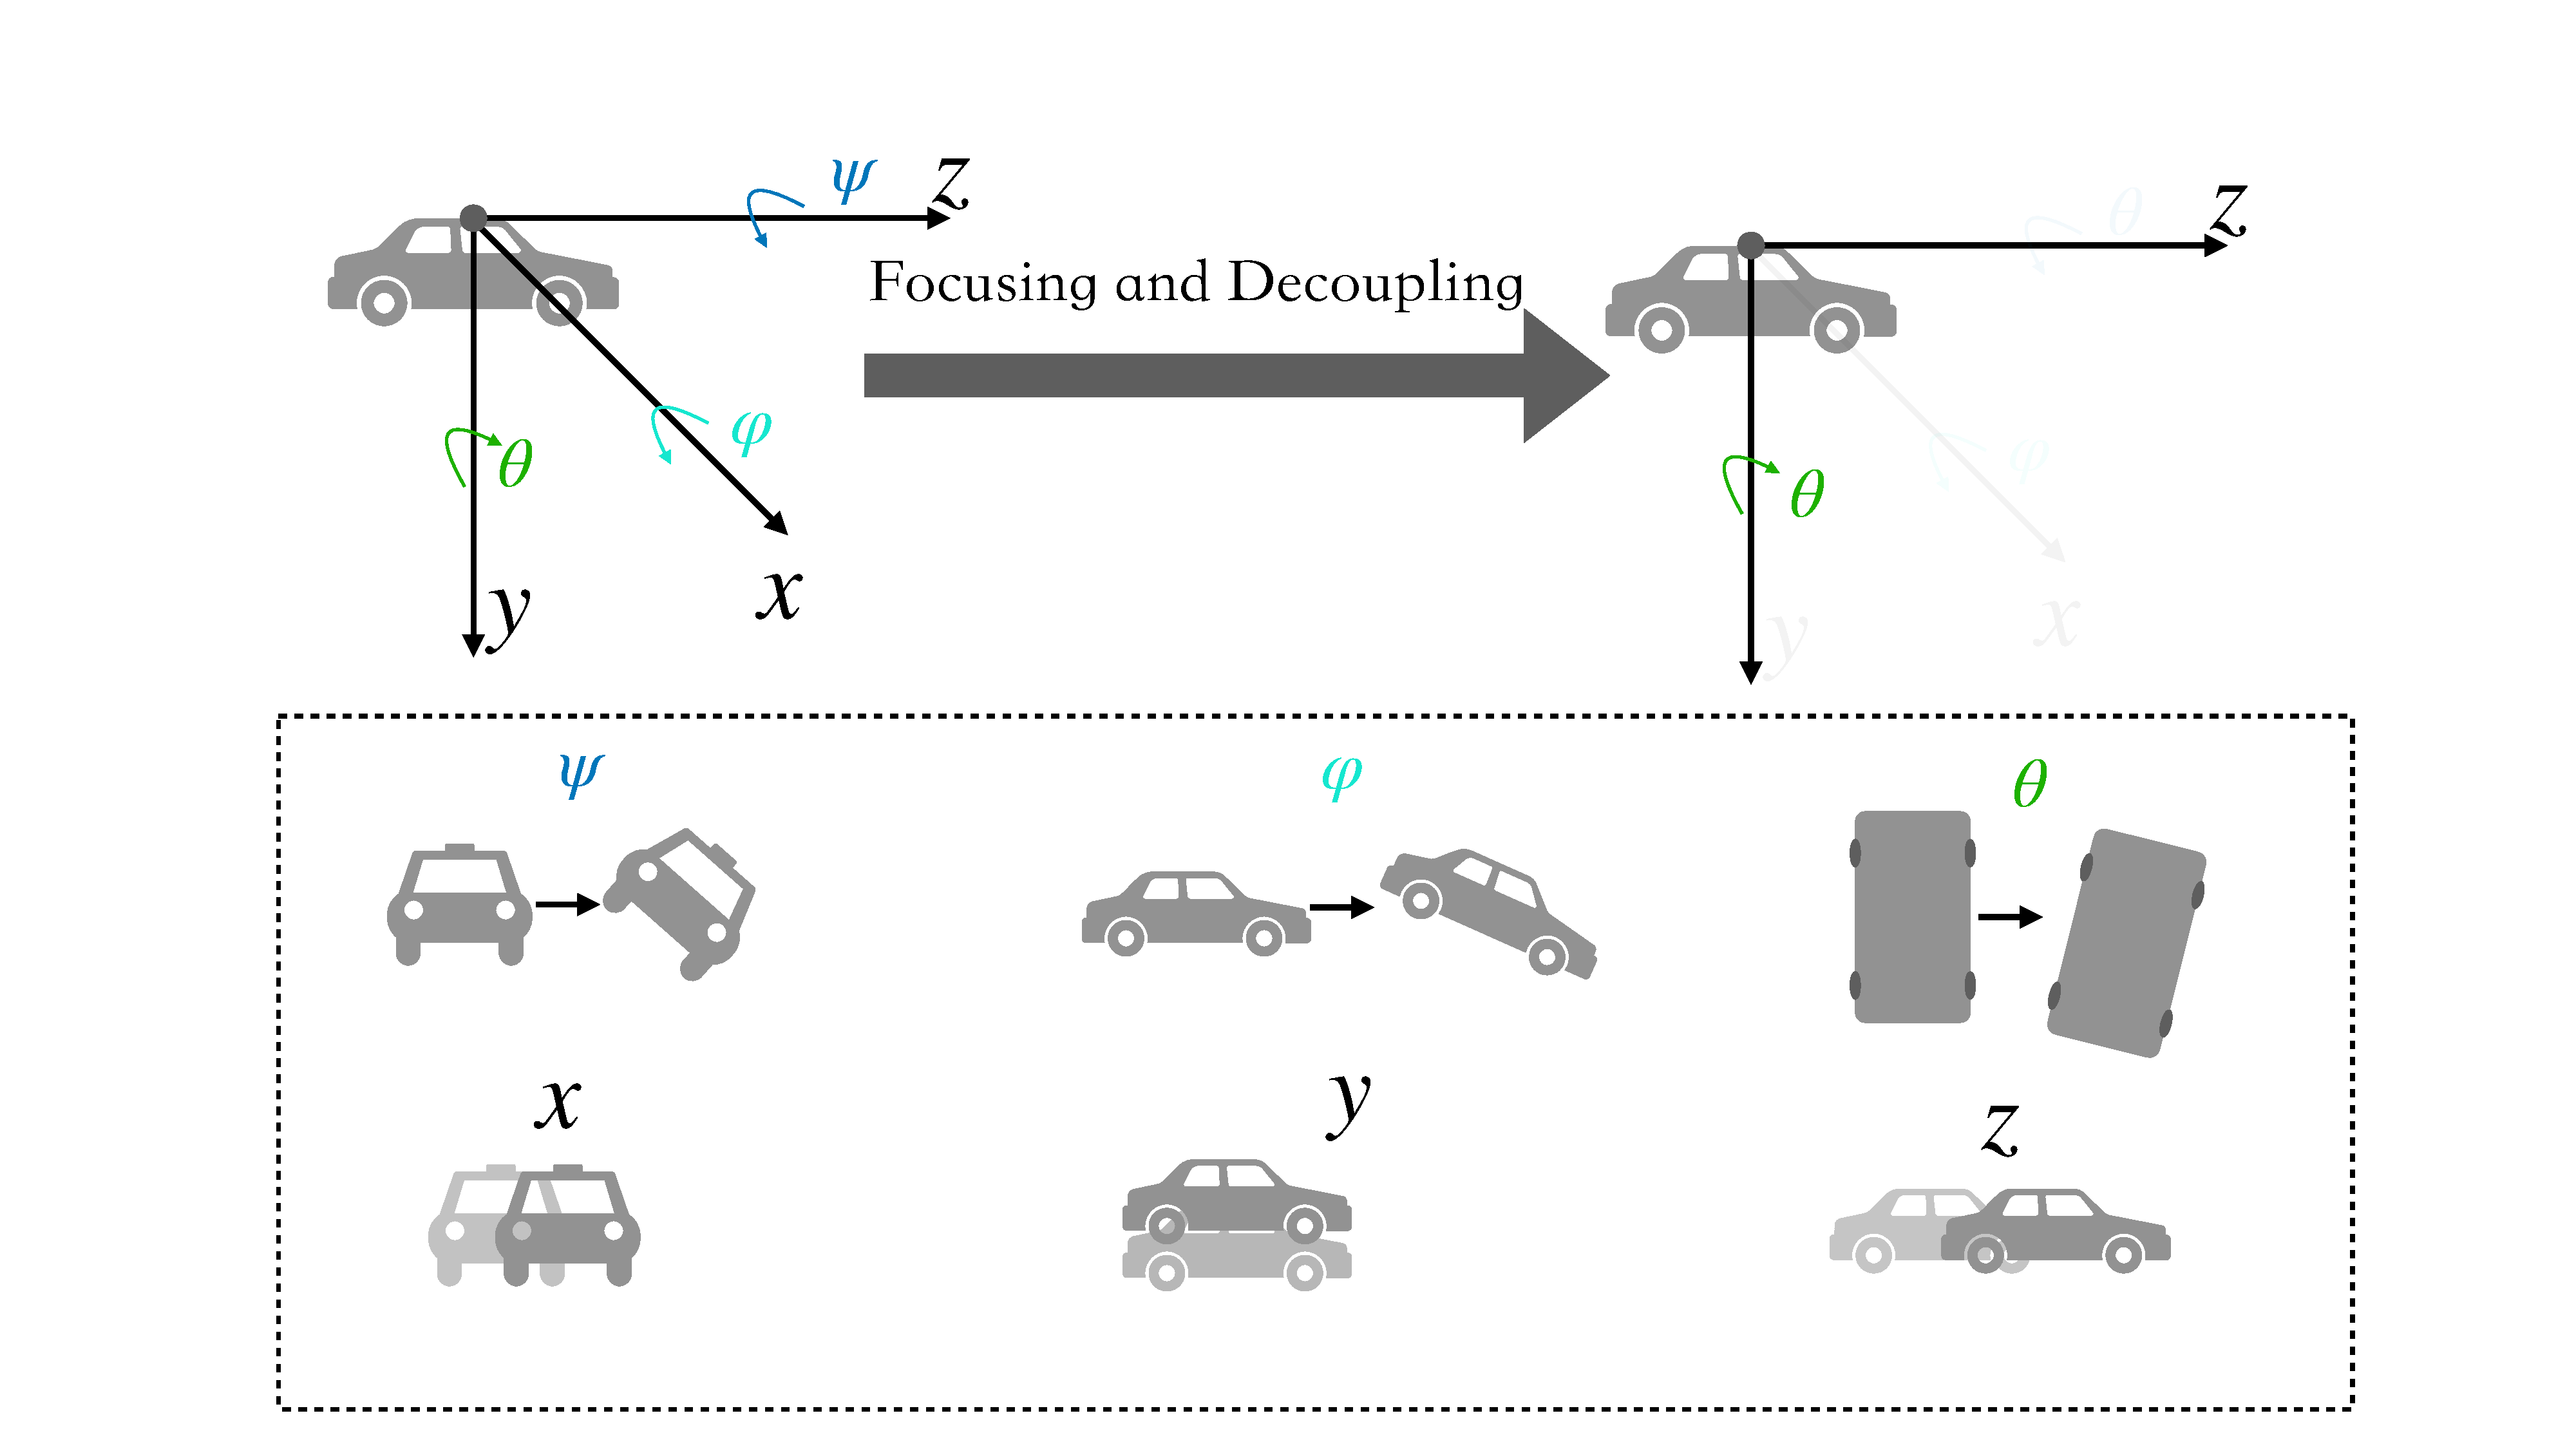
\includegraphics[width=0.7\textwidth]{datavo/car_simplify.pdf}
    \caption{Motivation: focusing on the majority motion of ground vehicle to simplify the learning target.}
    \label{fig:car_simplify}
\end{figure}

本文首先定量评估了忽略一些不显著运动维度所造成的姿势位移(命名为运动聚焦),并探讨了通过考虑地面车辆运动模型(命名为运动解耦)来最小化姿势位移。此外,
我们构建了仅有四个卷积层的轻卷积神经网络来学习地面车辆的显著运动,并进行了实验,表明运动聚焦运动解耦可以提高自我运动估计性能。整个系统的结构如图\ref{fig:system_structure}所示。
本文的主要贡献有:
\begin{enumerate}
    \item {通过对运动聚焦引起的地面真实姿势位移进行定量评估,发现其位移相对较小,可以通过实验证明运动聚焦的可行性。}
    \item {分析了X轴意外平移的原因,建立了X轴平移和Y轴旋转的关系模型,并利用该模型来减少运动解耦引起的姿势位移。}
    \item {我们在KITTI数据集上进行了对比实验,表明所提出的运动聚焦和解耦可以减少训练时间,提高学习性能。}
    \item {构建了轻型卷积神经网络来模拟地面车辆的主要运动,模型足够轻,可以在GPU上用2G左右的内存进行训练。并在CPU上实时运行(每秒超过200帧)。
    为了更好促进视觉里程计技术的发展,我们发布了项目源代码\footnote{https://github.com/TimingSpace/DMVOGV}。}
\end{enumerate}

\section{方法}
\label{sec:approach}
\subsection{运动聚焦与解耦}
\label{sec:motion}
运动聚焦是通过将注意力集中在大多数运动上来简化学习目标的一般思想,这在第\ref{sec:motion_focus}节有详细中描述,运动聚焦引起的姿势位移在节\ref{sec:info_loss}中评估。
运动解耦是为了减少运动聚焦引起的姿势位移,这在第\ref{sec:motion_decouple}节中描述,在\ref{sec:info_decouple}节中进行性能评估,运动聚焦和运动解耦所引起的学习改进将在\ref{sec:ego_improvement}中进行评价。
\begin{figure*}[t]
    \centering
    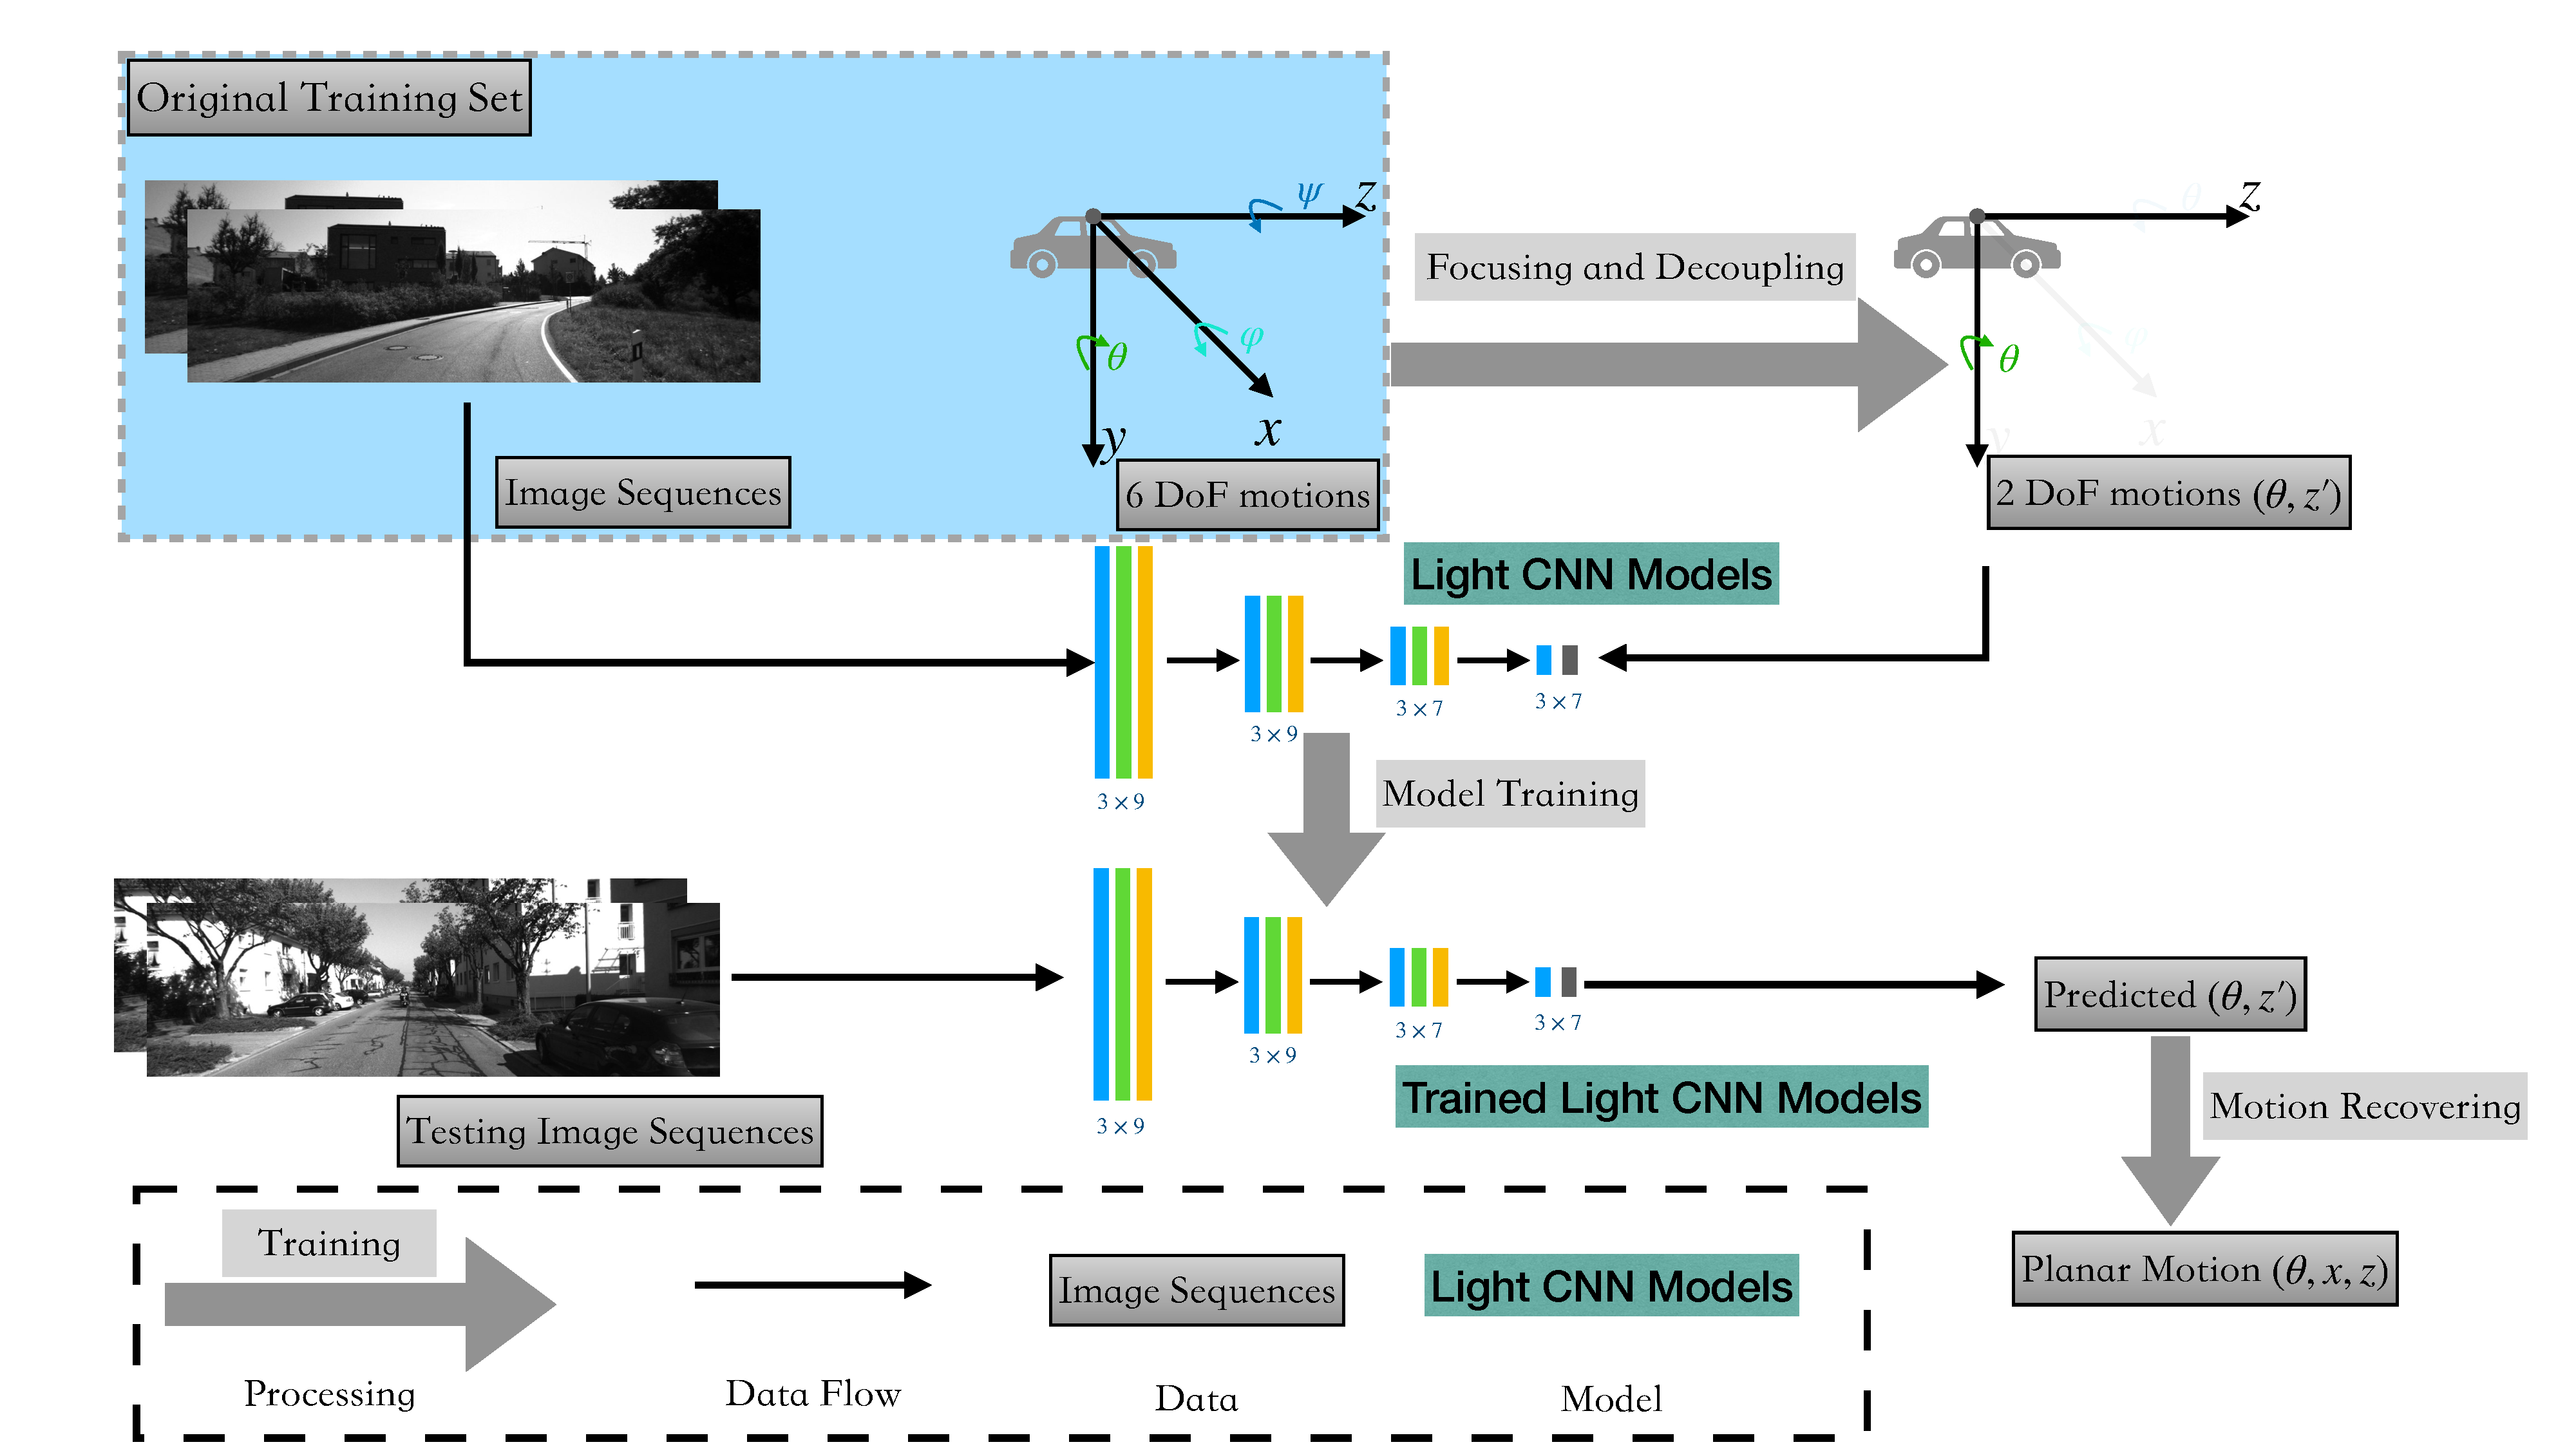
\includegraphics[width=0.9\textwidth]{datavo/system_structure.pdf}
    \caption{The structure of the whole system.}
    \label{fig:system_structure}
\end{figure*}

\subsubsection{运动聚焦}
\label{sec:motion_focus}
\begin{figure}[ht]
    \centering
    \begin{subfigure}[b]{0.225\textwidth}
        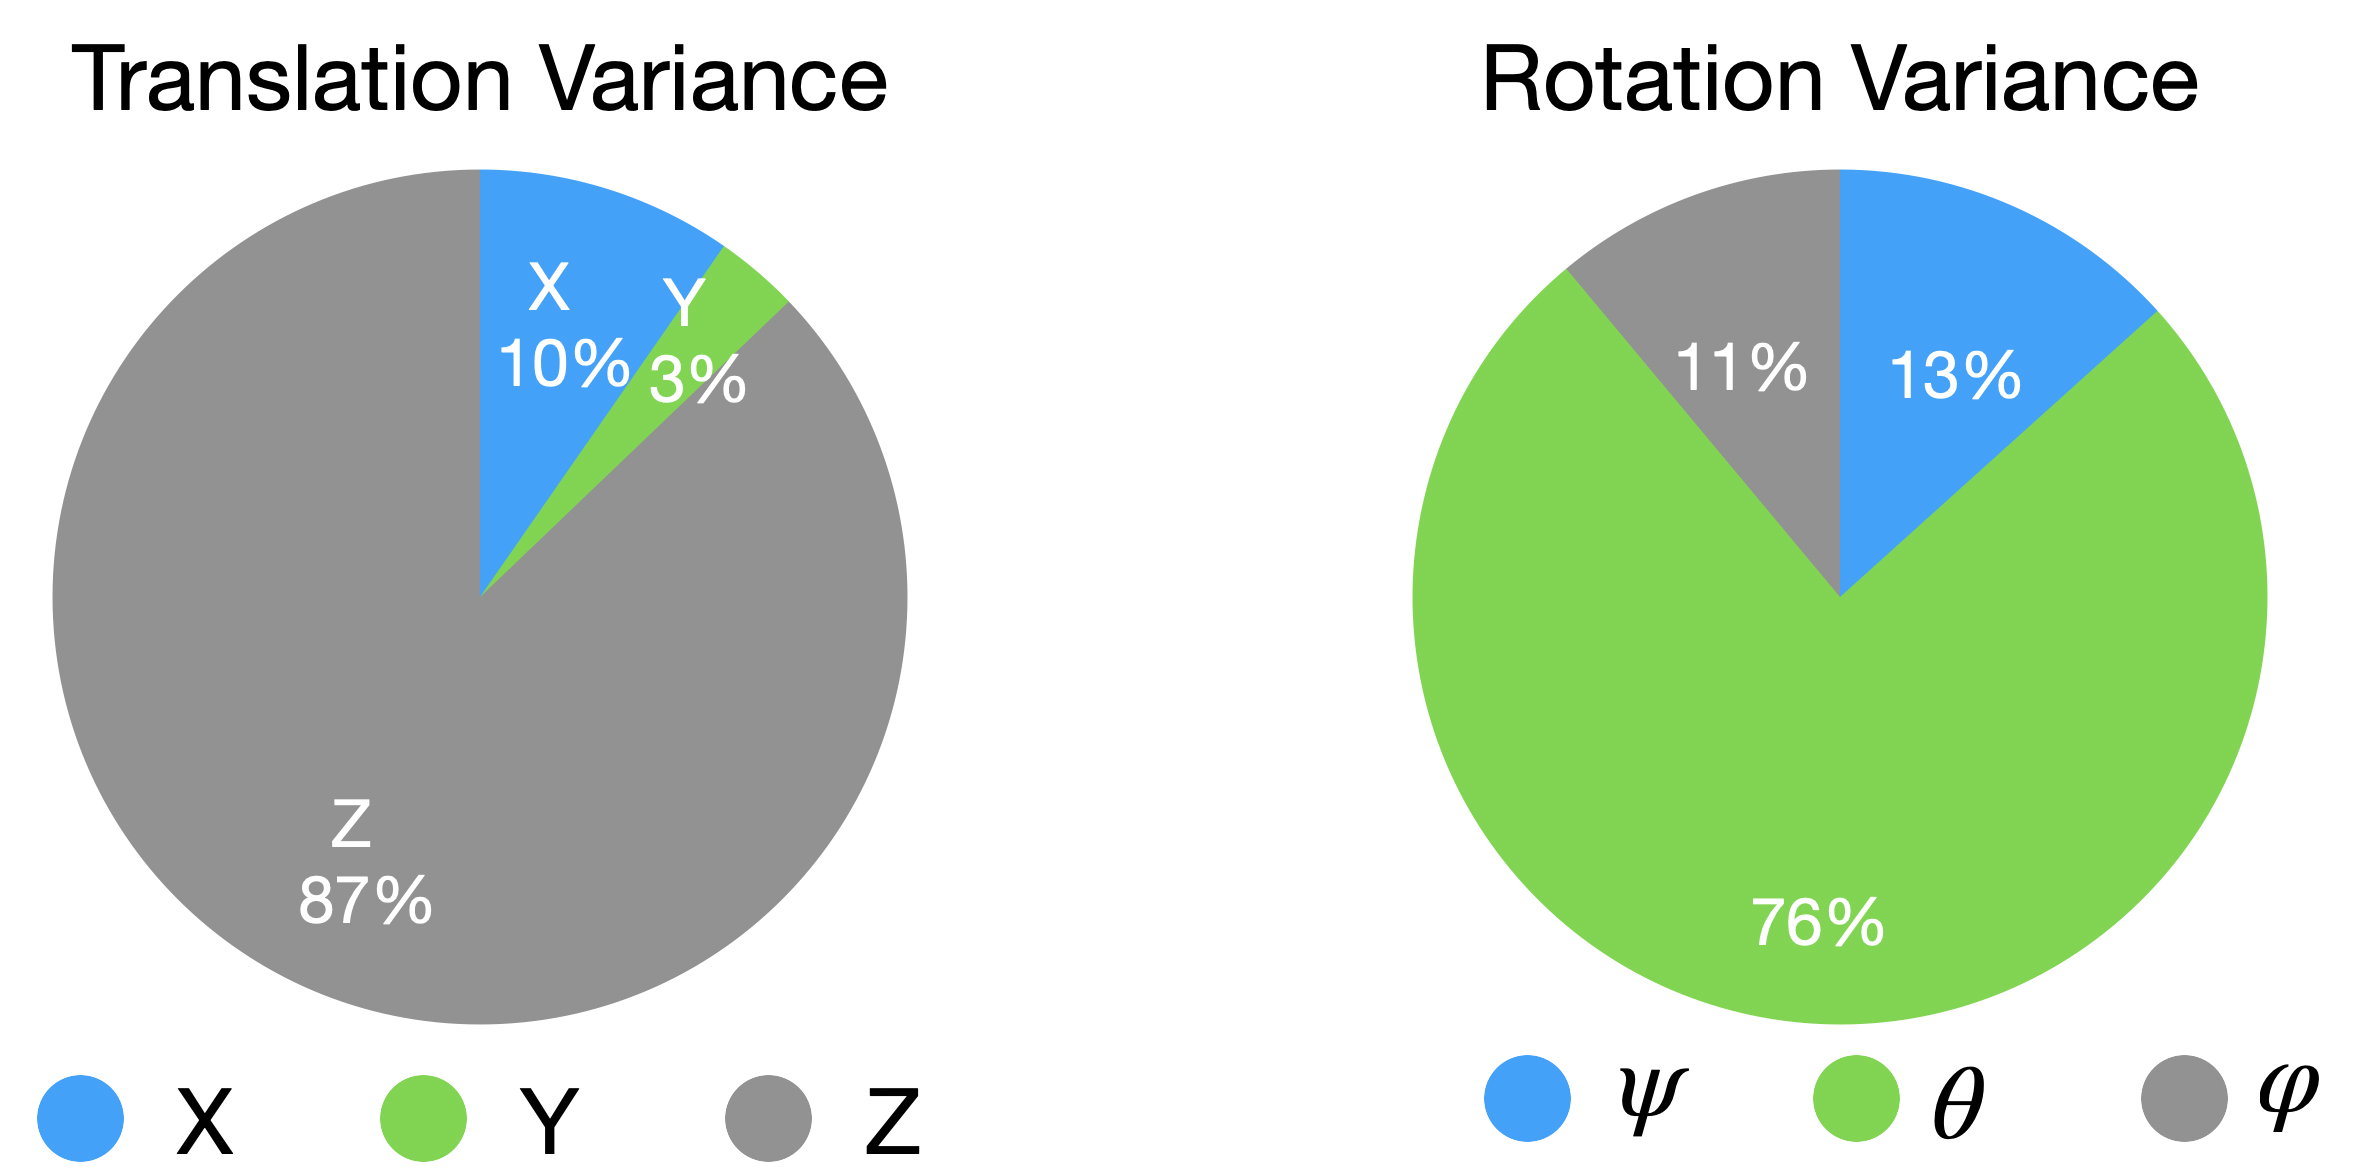
\includegraphics[width=\textwidth]{datavo/motion_dis.png}
        \caption{}
        \label{fig:motion_dis} 
    \end{subfigure}
    \begin{subfigure}[b]{0.225\textwidth}
        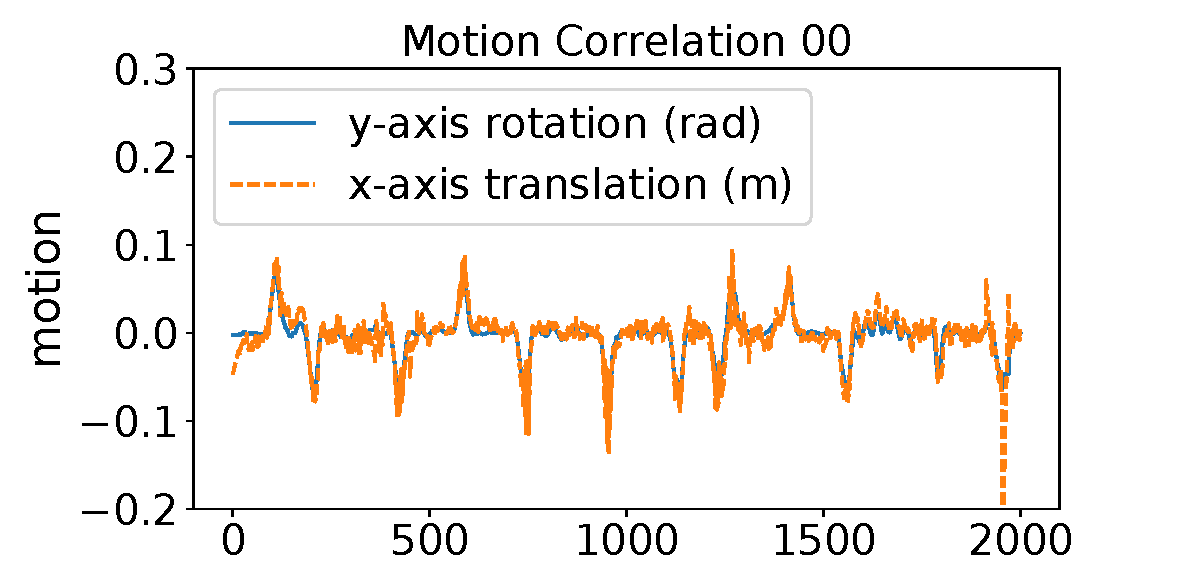
\includegraphics[width=\textwidth]{datavo/rotation_corr.pdf}
        \caption{}
        \label{fig:rotation_corr}
    \end{subfigure}
    \caption{Motion pattern analysis. (a) Comparison of the motion 
    along/about different axis; (b) Correlation of x-axis translation and y-axis rotation.}
\end{figure}

常见的处理运动幅度差的方法是数据归一化或采用不同的尺度恢复参数\cite{wang2017deepvo}。但由于地面车辆的约束运动轴的信噪比很小,归一化会引入大量的噪声。
运动聚焦是忽略地面车辆的微不足道的运动,集中精力对大部分运动进行建模。在分解运动时,我们使用常规的相机坐标系作为参考系(如图\ref{fig:car_simplify}所示),
它是一个右手系,定义如下:原点为相机的光学中心,z轴定义为前进的光轴,x轴为水平向右,y轴为垂直向下。
围绕x轴、y轴和z轴的旋转运动分别用Euler角$\psi$、$\varphi$和$\theta$表示,沿不同轴的平移运动分别用$x$、$y$和$z$表示。

\begin{figure}[h]
    \centering
    \begin{subfigure}[b]{0.225\textwidth}
        \centering
        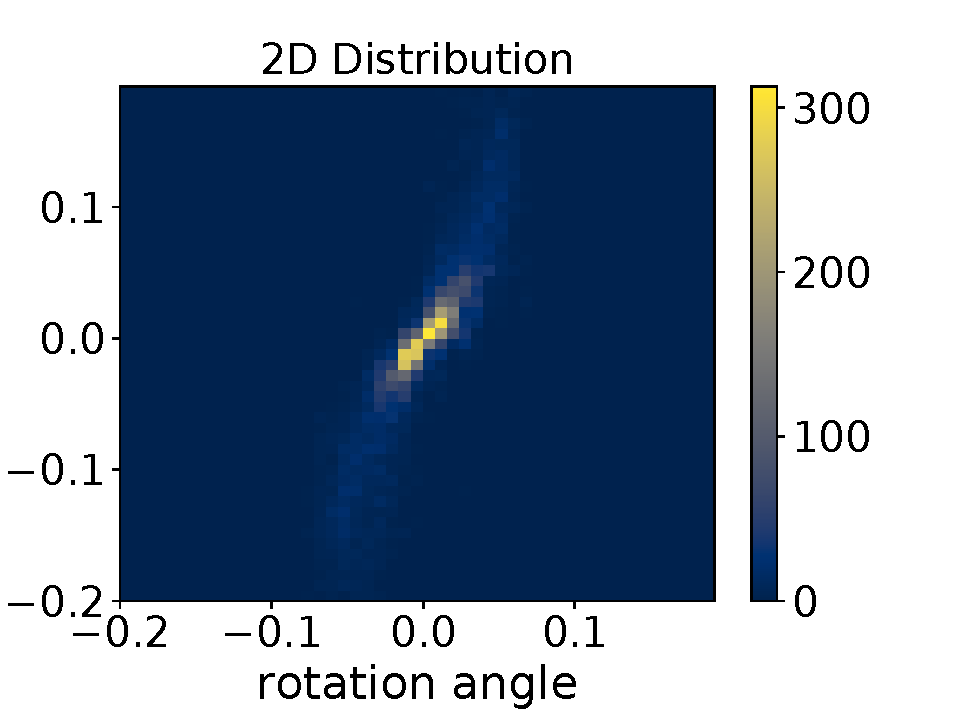
\includegraphics[width=\textwidth]{datavo/r_t_2d_hist.pdf}
        \caption{}
        \label{fig:rt_2d} 
    \end{subfigure}
    \begin{subfigure}[b]{0.225\textwidth}
        \centering
        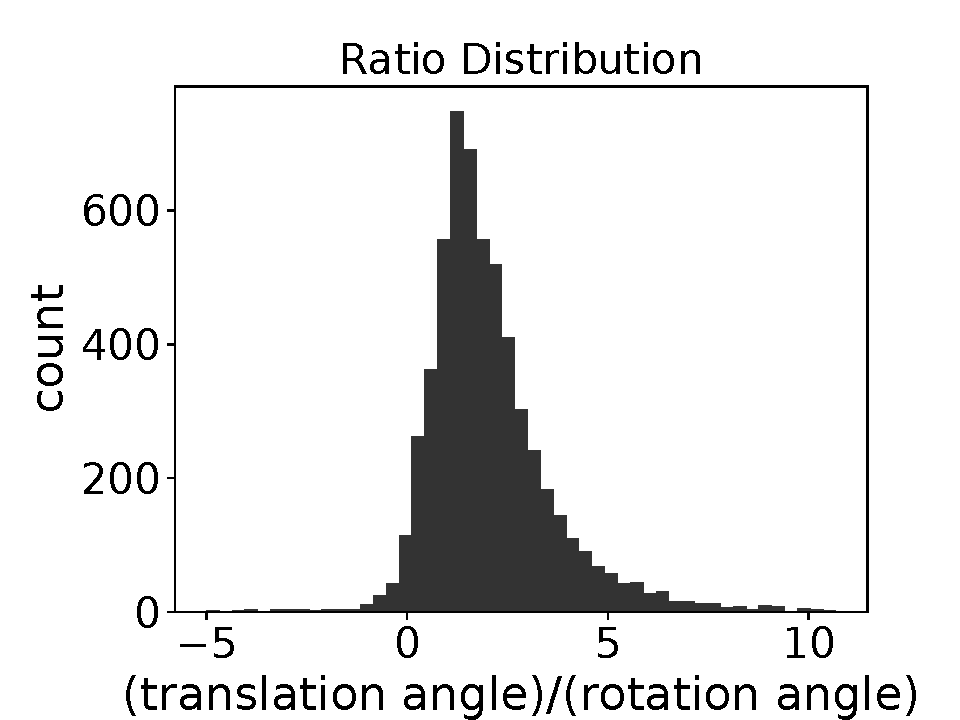
\includegraphics[width=\textwidth]{datavo/r_t_1d_hist.pdf}
        \caption{}
        \label{fig:rt_1d}
    \end{subfigure}
    \caption{Correlation of rotaion angle and translation angle. (a) 2D Histogram of translation angle and rotation angle; (b) 1D Histogram  of translation angle over rotation angle.}
    \label{fig:rotation_corr_analysis}
\end{figure}

我们在KITTI视觉里程计测评数据集\cite{geiger2012kitti}上对地面车辆的运动模式进行了定量评估。这是一个典型的路面车辆运动估计数据集。我们计算了KITTI序列00中关于不同轴
的平移运动和旋转运动的方差,如图\ref{fig:motion_dis}所示,%更多的方差可视化可以在补充中获得,这与图\ref{fig:motion_dis}类似}。
由该图可知地面车辆的大部分运动是z轴平移和y轴旋转。所以我们建议简化运动估计目标,只关注大多数运动,我们称这个建议为运动聚焦。由运动聚焦引起的姿势位移在第\ref{sec:info_loss}节中进行评估。
运动解耦是为了减少由运动聚焦引起的姿势位移,这在第\ref{sec:motion_decouple}节中描述,在第\ref{sec:info_decouple}节中评估。
运动聚焦和运动解耦引起的学习改进在第\ref{sec:ego_improvement}节中进行评估。


\subsubsection{运动解耦}
\label{sec:motion_decouple}
尽管如此,沿x轴仍存在不可忽略的平移运动,如图\ref{fig:motion_dis}所示。结合表\ref{tab:info_loss_1}分析,
我们可以知道,如果忽略X轴的运动,会造成更多的漂移姿势,但考虑到动力学约束,地面车辆不能沿X轴移动太多。
然而,考虑到动力学约束,地面车辆不能沿x轴移动太多,那如何获得10%的X轴位移?
当深入研究地面车辆的运动模式时。我们发现,X轴的运动是由以下运动表示方法引起的:
\begin{equation}
    \begin{pmatrix} \mathbf{R} & \mathbf{t}\\ 0 & 1  \end{pmatrix} = \begin{pmatrix} \mathbf{I}& \mathbf{t}\\ 0 & 1  \end{pmatrix}\begin{pmatrix} \mathbf{R}& \mathbf{0}\\ 0 & 1  \end{pmatrix}
    \label{eq:ftlr}
\end{equation}
其中$\mathbf{I}$是一个3x3的身份矩阵。在这个表示方法中, 平移运动$\mathbf{t}$先于旋转运动$\mathbf{R}$。因此,当车辆有旋转运动时,参考坐标系已经发生了改变,前向运动{$z'$}被映射成较小的前向运动{$z$}与侧向运动(x轴平移{$x$}),如图\ref{fig:vehicel_rotation_model}所示。
它引起的平移角$\alpha$,定义为 
\begin{equation}
    \alpha = \arctan\left(\frac{x}{z}\right)
\end{equation}


其中$x$和$z$分别代表x轴平移和z轴平移。当我们将x轴平移和y轴旋转可视化后(如图\ref{fig:rotation_corr}所示),就可以得到验证,因为这两个运动是高度相关的。

图\ref{fig:rotation_corr}只能可视化一个子序列的局部相关性。我们利用图中的两个直方图(\ref{fig:rotation_corr_analysis})来可视化所有KITTI序列00-10中所有Y轴
旋转角$\theta$和平移角$\alpha$的全局关系。图\ref{fig:rt_1d}中的1d直方图显示了$\alpha/\theta$的分布,图\ref{fig:rt_2d}中的2d直方图可视化了$\alpha$和$\theta$
的联合分布。这两个分布都表明y轴的旋转角$\theta$和平移角$\alpha$是相关的。那么如何对该运动进行数学建模以减少运动的相关性呢?一个简便的方法是将平移重写为
\begin{equation}
    \begin{pmatrix} \mathbf{R} & \mathbf{t}\\ 0 & 1  \end{pmatrix} = \begin{pmatrix} \mathbf{R'}& \mathbf{0}\\ 0 & 1  \end{pmatrix}\begin{pmatrix} \mathbf{I}& \mathbf{t'}\\ 0 & 1  \end{pmatrix}
    \label{eq:frlt}
\end{equation}
在这个公式中,车辆的旋转先于平移,所以平移运动是相对于旋转运动后的参考系而言的,不会被重新映射。可以得出以下关系:
$\mathbf{R'} = \mathbf{R}$, $\mathbf{t'} = \mathbf{R}^{-1}\mathbf{t}$.
\begin{figure}[ht]
    \centering
    \begin{subfigure}[b]{0.45\textwidth}
        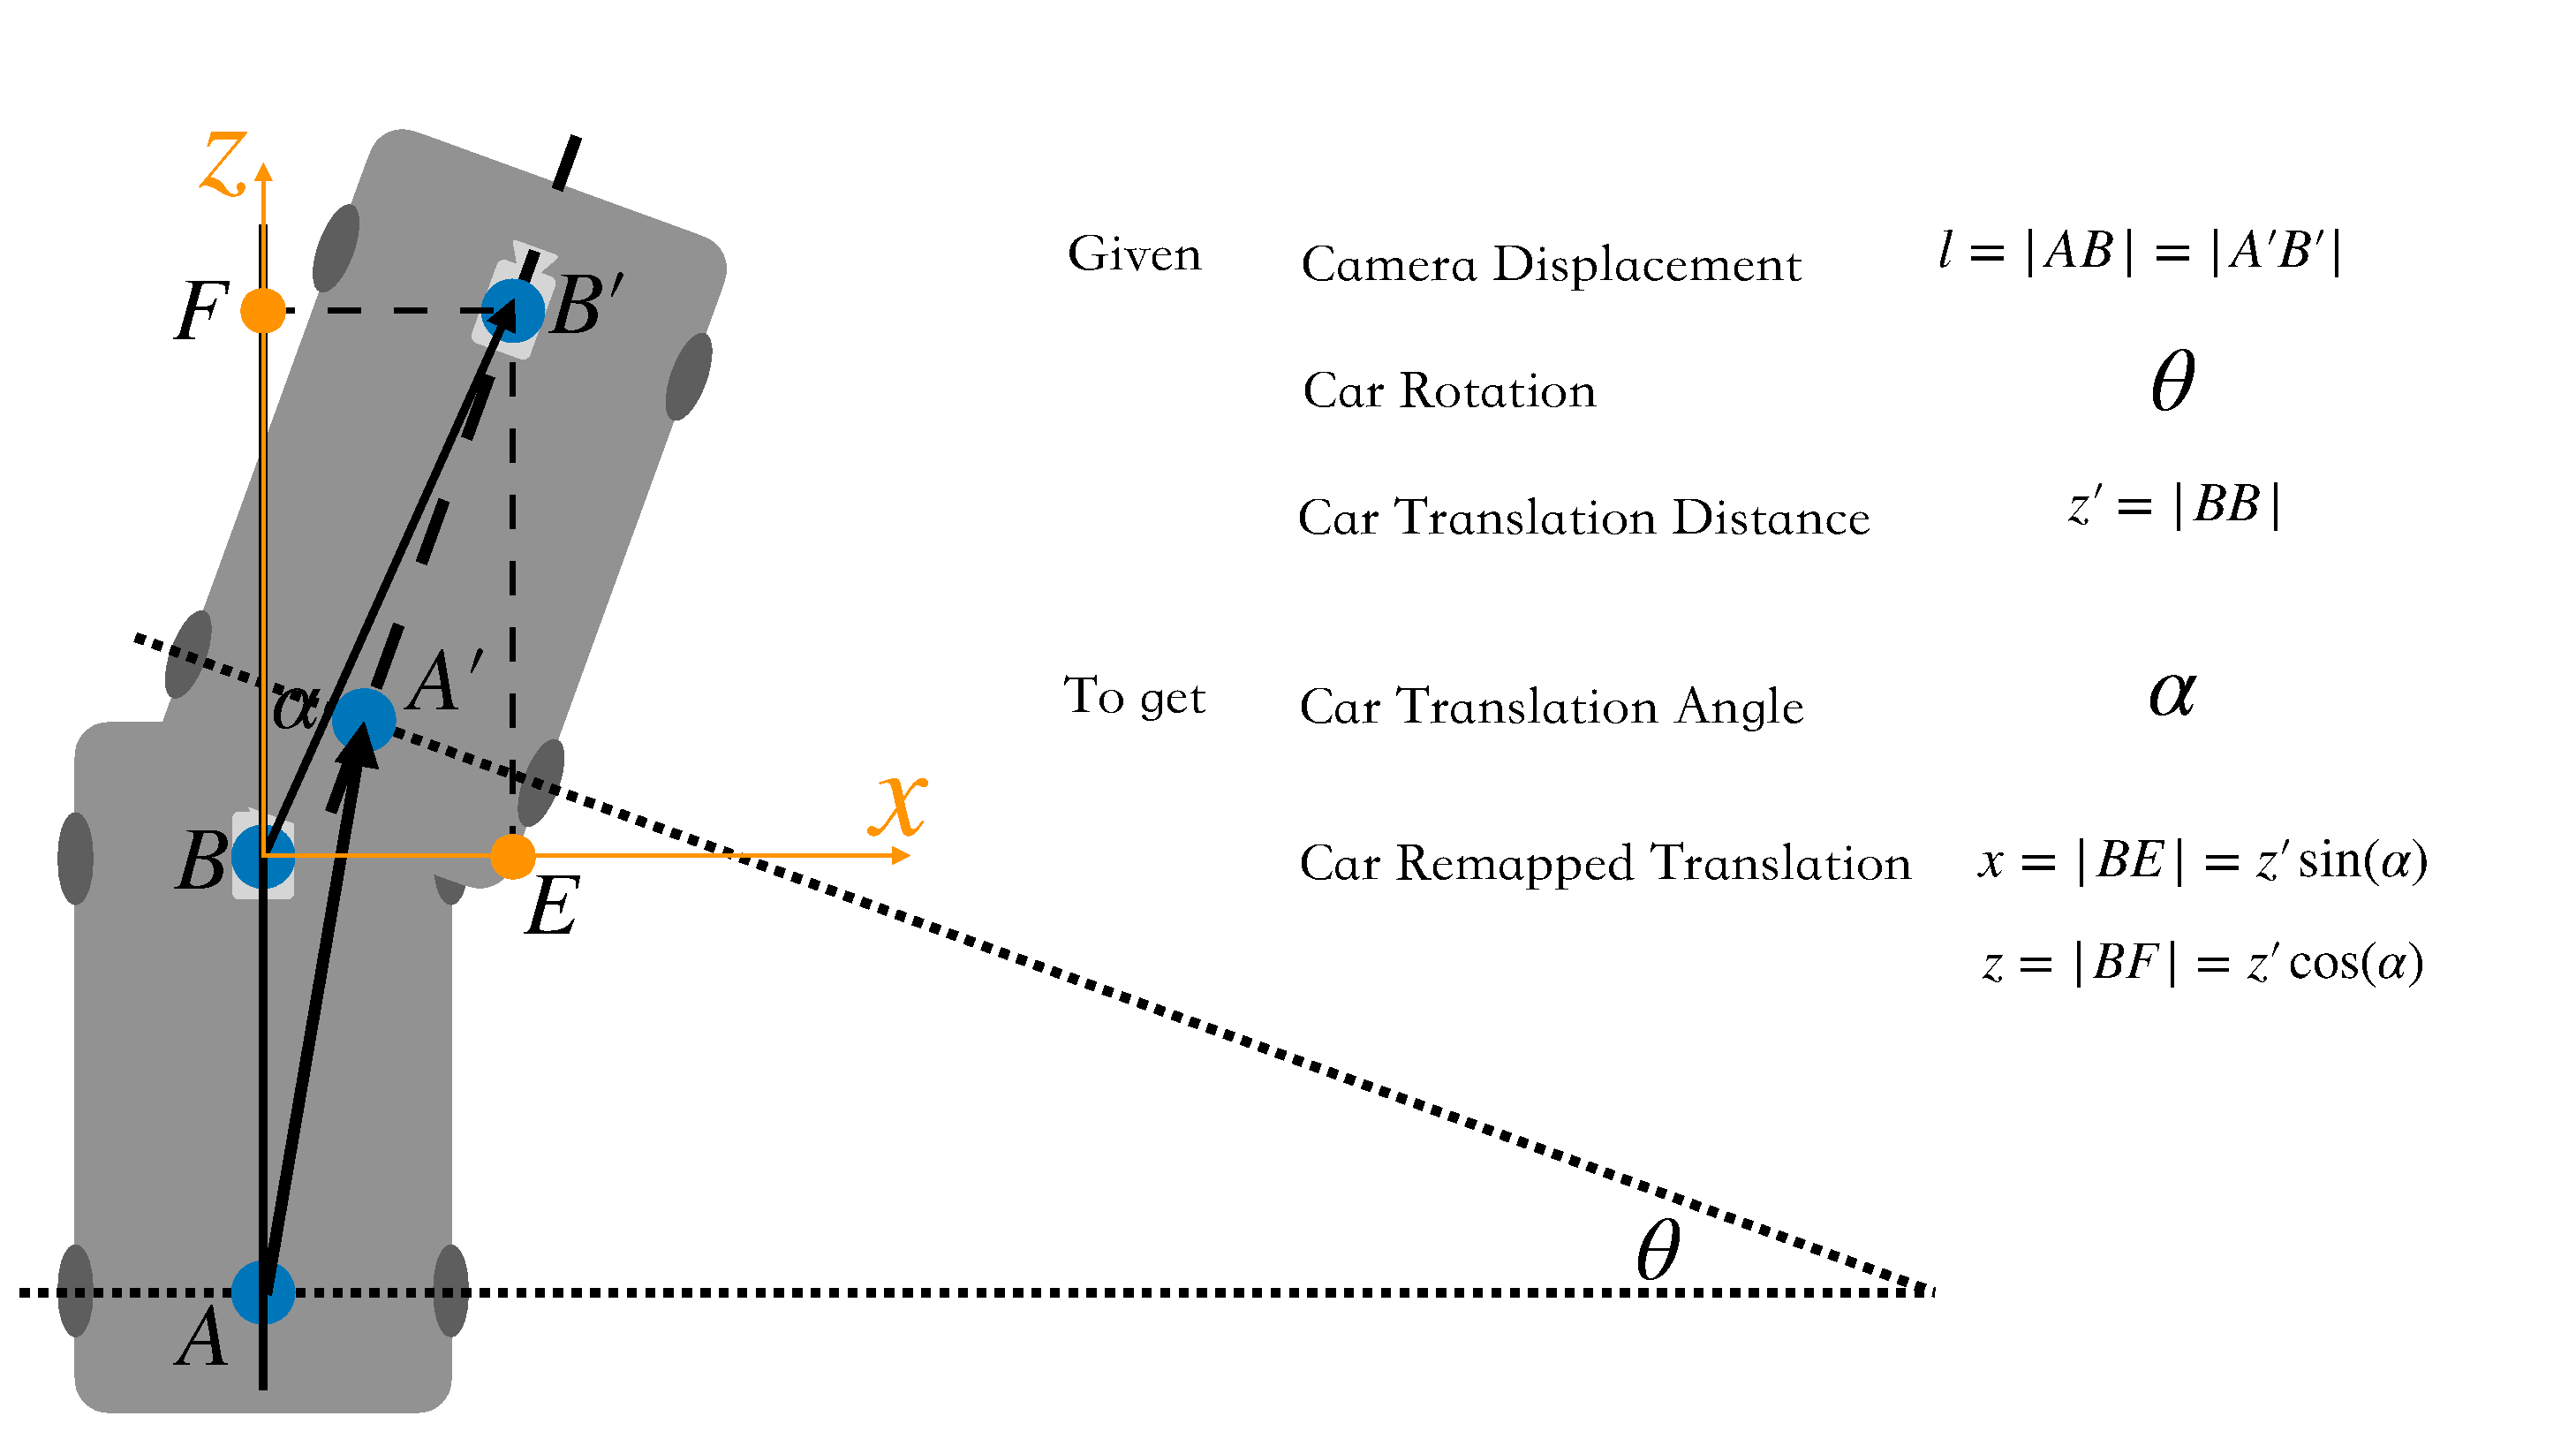
\includegraphics[width=\textwidth]{datavo/vehicle_rotation_1-crop.pdf}
        \caption{}
        \label{fig:vehicel_rotation_model} 
    \end{subfigure}
    \begin{subfigure}[b]{0.45\textwidth}
        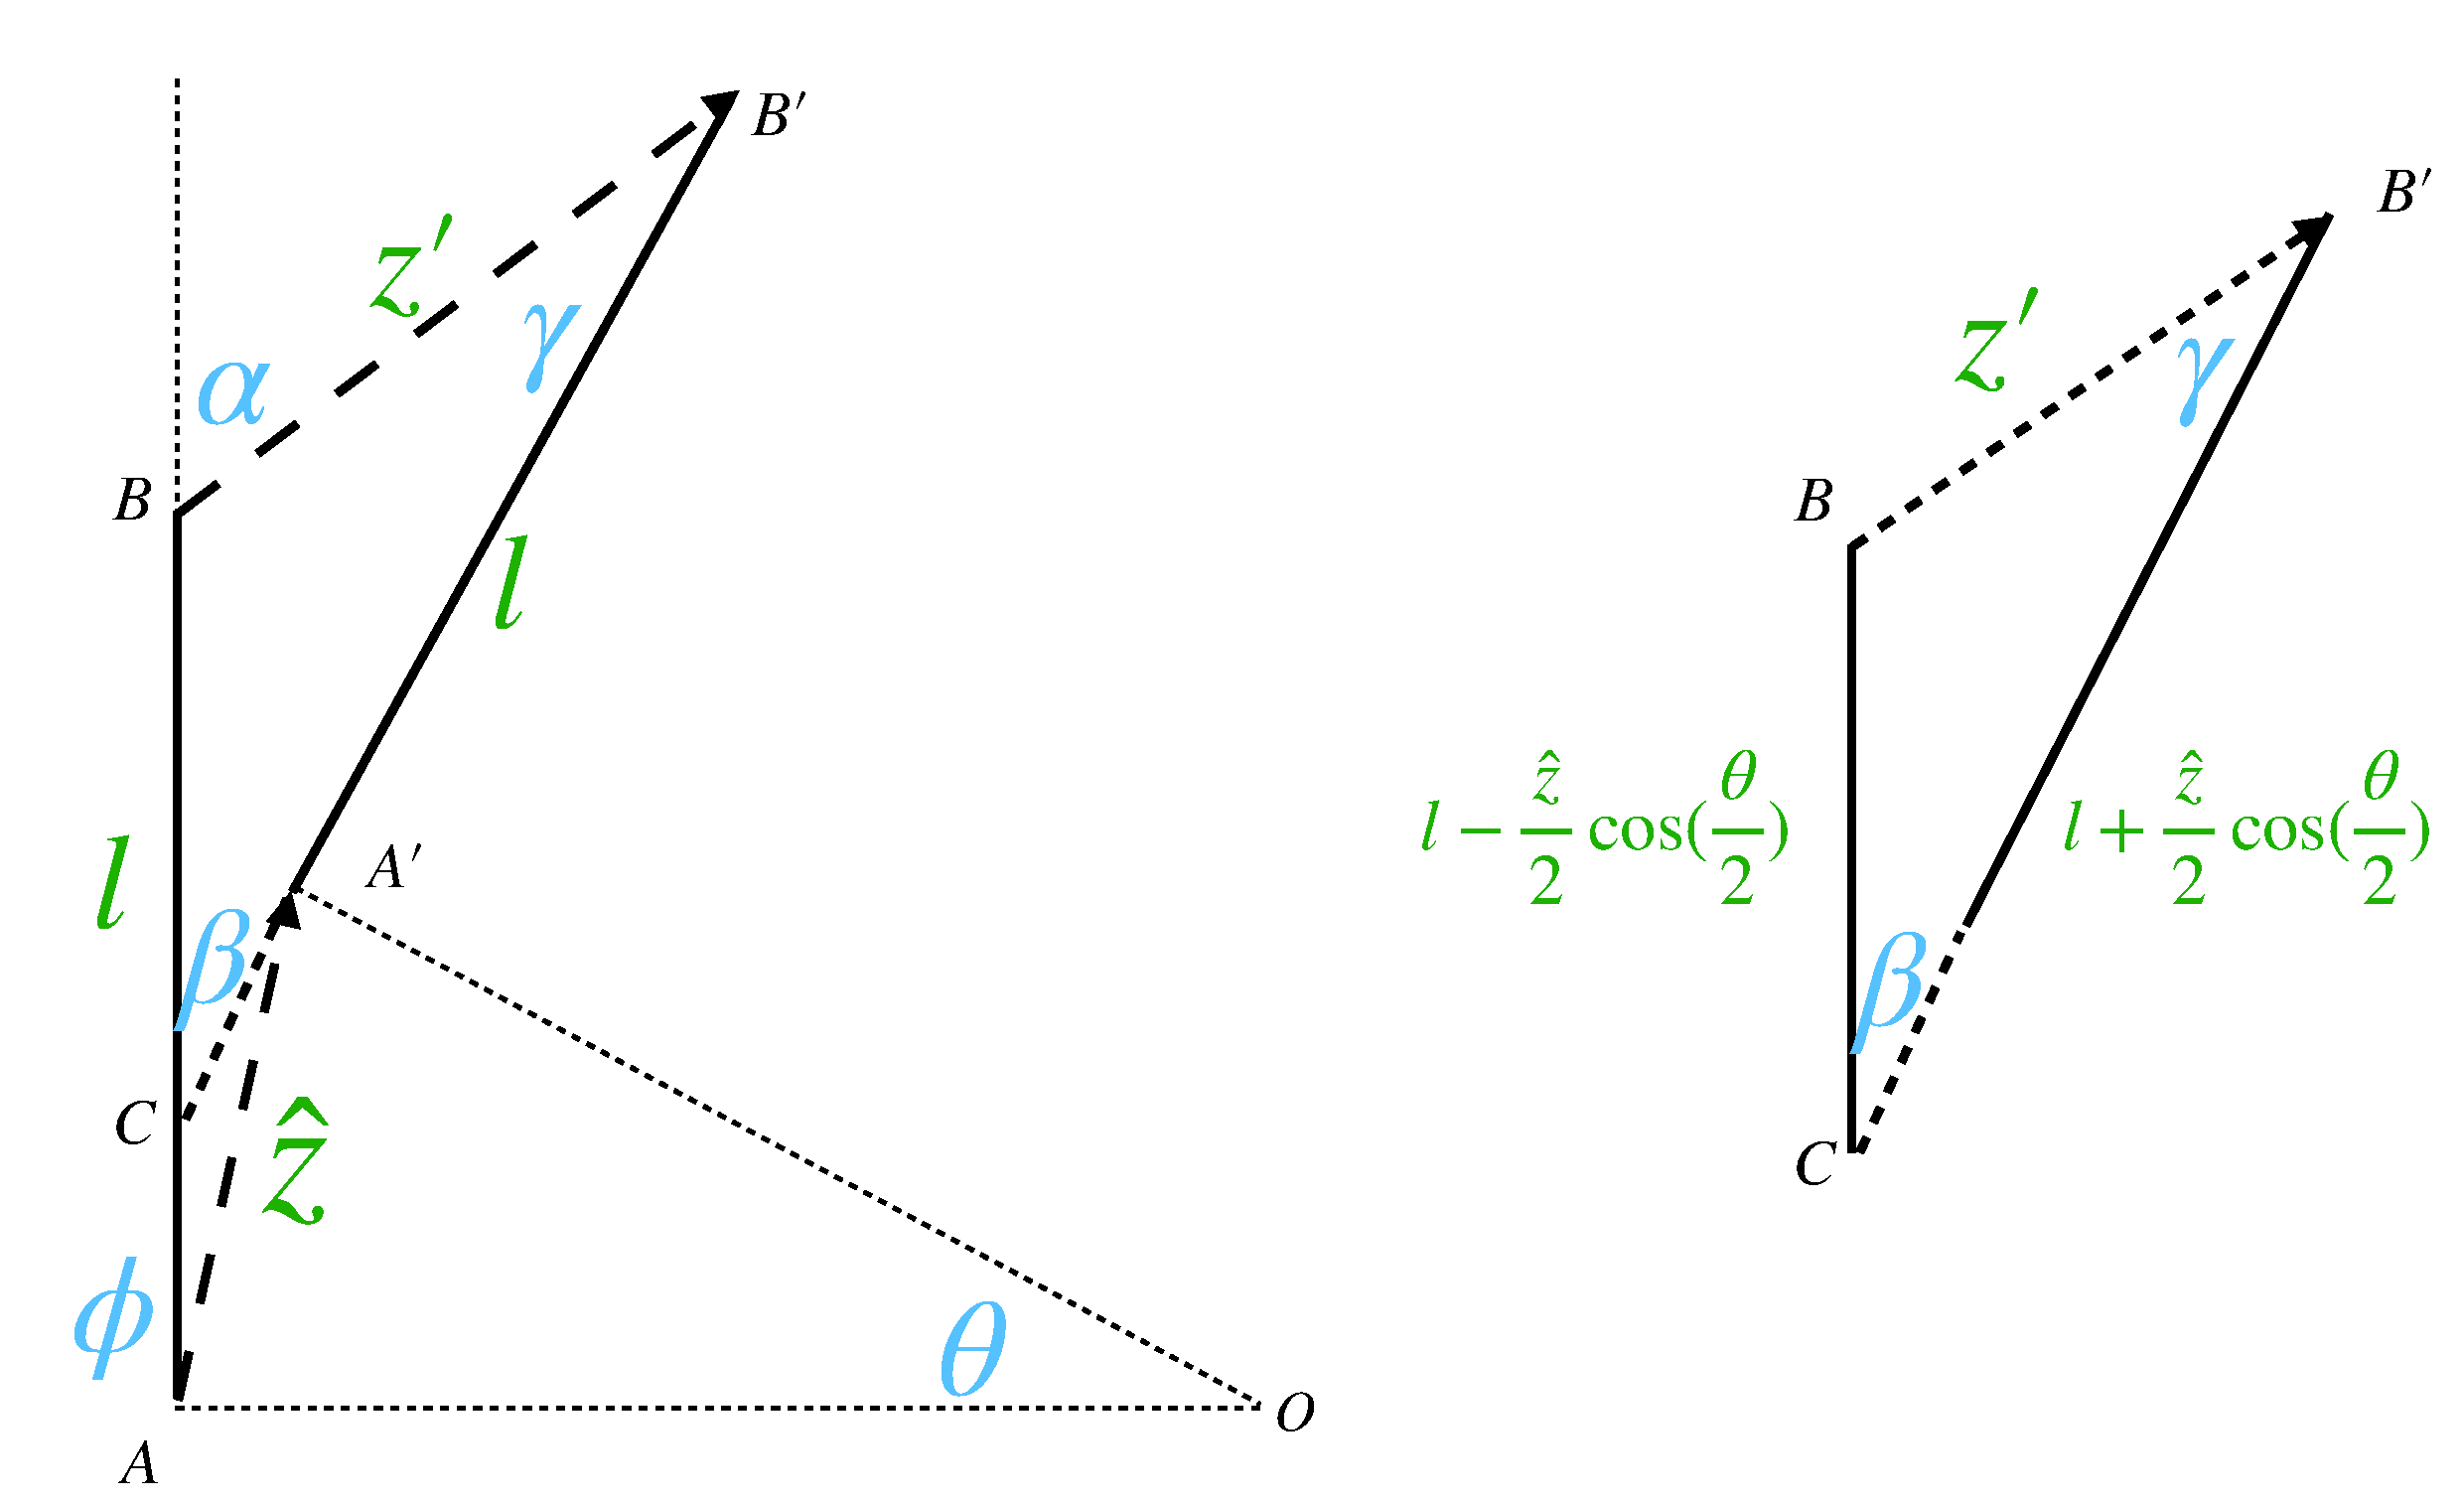
\includegraphics[width=\textwidth]{datavo/vehicle_rotation_2-crop.pdf}
        \caption{}
        \label{fig:vehicel_rotation_model_s} 
    \end{subfigure}
    \caption{Ground vehicle rotation model. (a) Rotation model; (b) Simplified rotation model.}
    \label{fig:rotation_model}
\end{figure}

然而,如图\ref{fig:vehicleel_rotation_model}所示,绕y轴的旋转角$\theta$不等于旋转产生的平移角$\alpha$。我们需要找出$\alpha$和$\theta$之间的关系
$\alpha=f(\theta)$,然后我们可以利用位移角$\alpha$来恢复车辆的运动,只需保留y轴旋转$\theta$和车辆前行位移$z$:
\begin{equation}
    (x,z) = z'(sin(f(\theta)),cos(f(\theta)))
    \label{eq:car_angle}
\end{equation}
在图\ref{fig:vehicleicel_rotation_model}中,A是指车辆后轴的中心,而B是安装摄像头的位置。A和B之间的距离表示为$l$,表示摄像头的位置。通过视觉里程测量法估算出的车辆
平移距离为$B$和$B'$之间的距离,表示为$z'$。我们将图\ref{fig:vehicleicel_rotation_model}简化为图\ref{fig:vehicleel_rotation_model_s}。
根据阿克曼转向原理\cite{siegwart2011introduction},$OA\bot AB$,$OA'\bot A'B'$,所以$\phi=0.5 \beta=0.5 \theta$。

在三角形$CBB'$中,根据正弦定律,
\begin{equation}
   \frac{\sin(\gamma)}{\sin(\beta)}  = \frac{l-\frac{\hat{z}}{2} / \cos(\frac{\theta}{2})}{z'} 
\end{equation}
考虑到$\theta$接近于零,可以近似地认为$\cos(\frac{\theta}{2}) \approx1$,$\frac{\gamma}{\beta} \approx\frac{\sin(\gamma)}{\sin(\beta)}$,所以
\begin{equation}
    \frac{\gamma}{\beta}  \approx \frac{l-\frac{\hat{z}}{2}}{z'} 
\end{equation}
根据三角形余弦定理,在三角形$CBB'$中,{$d = |AC| \approx 0.5|AA'| =0.5\hat{z}$}, 
\begin{equation}
    \begin{split}
        z'^2 &= (l+d)^2 + (l-d)^2- 2(l+d)(l-d)\cos(\beta) \\
        &= 2l^2+2d^2 - 2(l^2-d^2)\cos(\beta)\approx 4d^2
    \end{split}
\end{equation}
因此$z'\approx\hat{z}$。那么平移角$\alpha$和旋转角$\theta$之间的关系是:
\begin{equation}
    \alpha = \beta + \gamma \approx (\frac{l}{z'}+0.5)\beta =(\frac{l}{z'}+0.5)\theta
    \label{eq:r_t_ratio}
\end{equation}
我们使用平移角$a$重构一个旋转矩阵$\mathbf{R}_\alpha$:
\begin{equation}
    \mathbf{R}_\alpha = \begin{pmatrix}
        \cos(\alpha)& 0 & \sin(\alpha)\\ 
        0 & 1 & 0\\ 
        -\sin(\alpha)& 0 & \cos(\alpha)\\ 
    \end{pmatrix} 
    \label{eq:r_alpha}
\end{equation}
因此$\mathbf{t}'$可转换为:
\begin{equation}
    \mathbf{t}' = \mathbf{R}_\alpha^{-1}\mathbf{t}
    \label{eq:decouple_z}
\end{equation}
所需的车辆前行运动{$z'$}是$\mathbf{t}'$的第三个元素。到目前为止,地面车辆的规划者运动可以由两个变量来表示:旋转角$\theta$和{重映射}前向运动{$z'$}。我们专注于学习二维
运动,以简化学习目标。模型和学习细节将在下一节介绍,运动聚焦和解耦引起的改进将在第\ref{sec:ego_improvement}节中评估。

\subsection{模型与训练}
\label{sec:model}
\begin{figure*}[t]
    \centering
    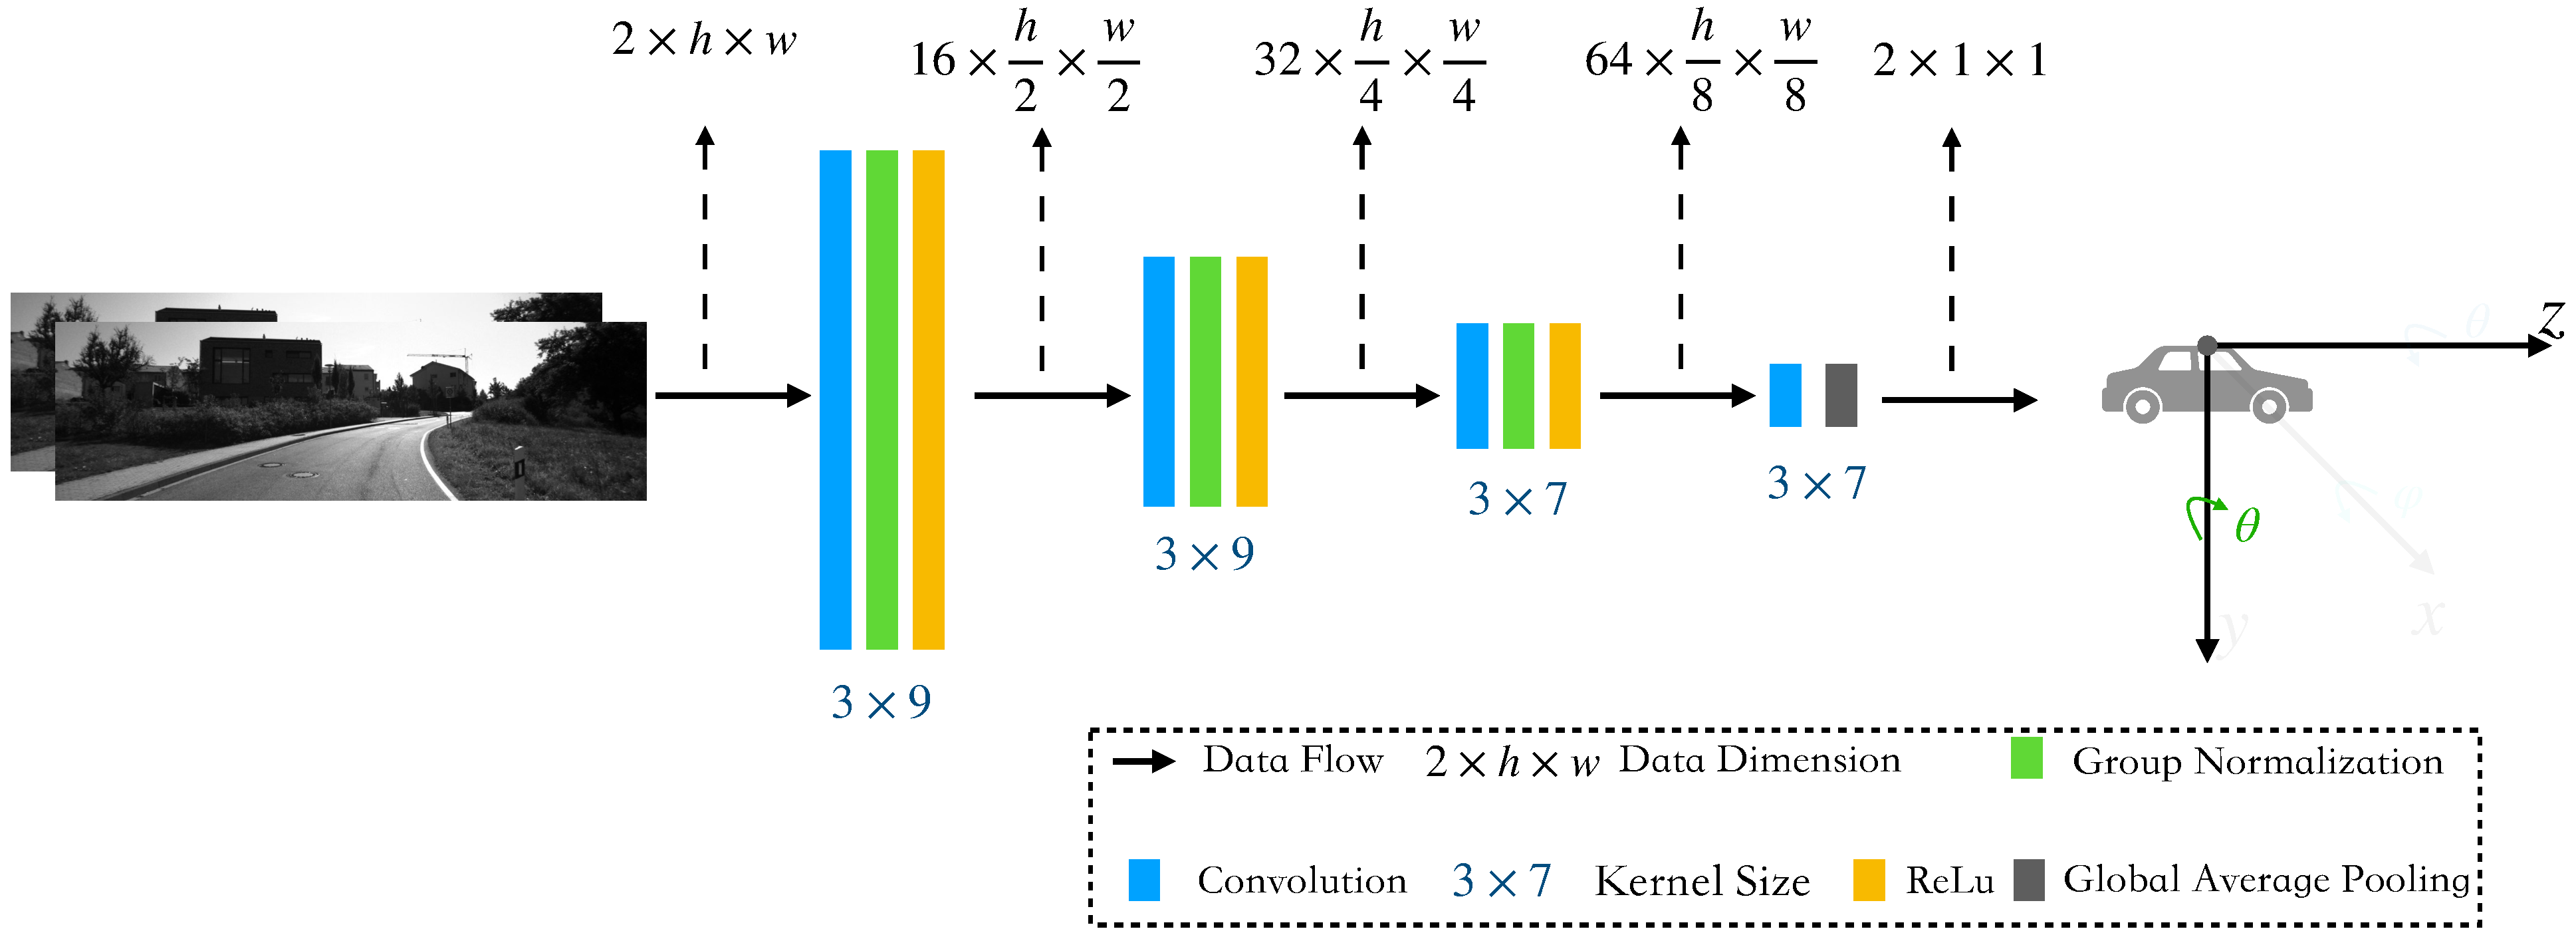
\includegraphics[width=0.9\textwidth]{datavo/network_structure_2-crop.pdf}
    \caption{自我位姿估计的轻便卷积神经网络。}
    \label{fig:nerwork_structure}
\end{figure*}
我们构建一个轻便模型来学习地面车辆的主要运动,如图\ref{fig:nerwork_structure}所示。
模型主要由卷积层构建,每个卷积层后面都有一个归一化层\cite{wu2018group}和ReLU{(整流线性单元)层}除外。与Zhou等人相同的是\cite{zhou2017unsupervised},
我们使用全局平均池层\cite{lin2013network}代替全连接层作为最后一层,以减少过拟合。我们观察到,地面车辆拍摄的图像的光流主要是水平的,特别是当车辆转弯时,如图
\ref{fig:optical_flow}所示。所以我们利用卷积层与非正方形核来实现{a}更大的水平感知场。此外,我们还采用了扩张卷积层\cite{yu2015multi},以较少的参数获得更大的感知场。

\begin{figure}[ht]
    \centering
    \begin{subfigure}[b]{0.45\textwidth}
        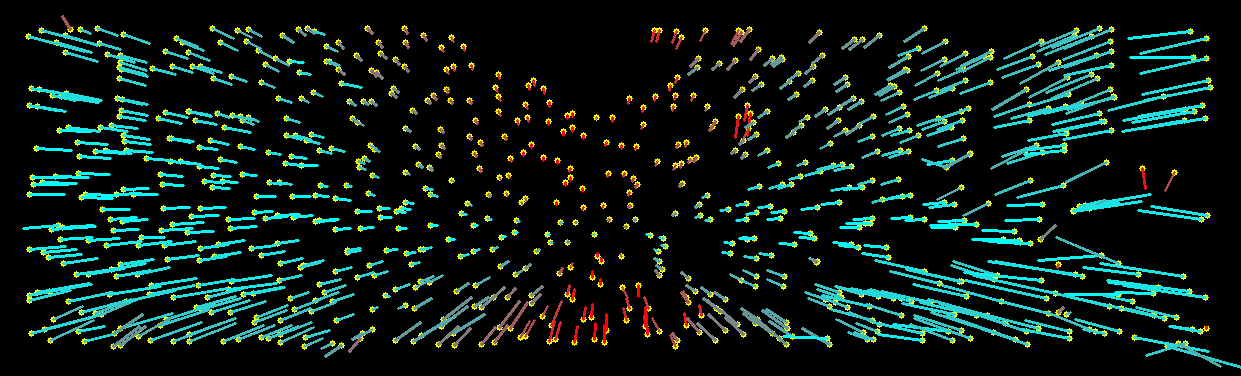
\includegraphics[width=\textwidth]{datavo/flow_61.png}
        \caption{}
        \label{fig:optical_flow_f} 
    \end{subfigure}
    \begin{subfigure}[b]{0.45\textwidth}
        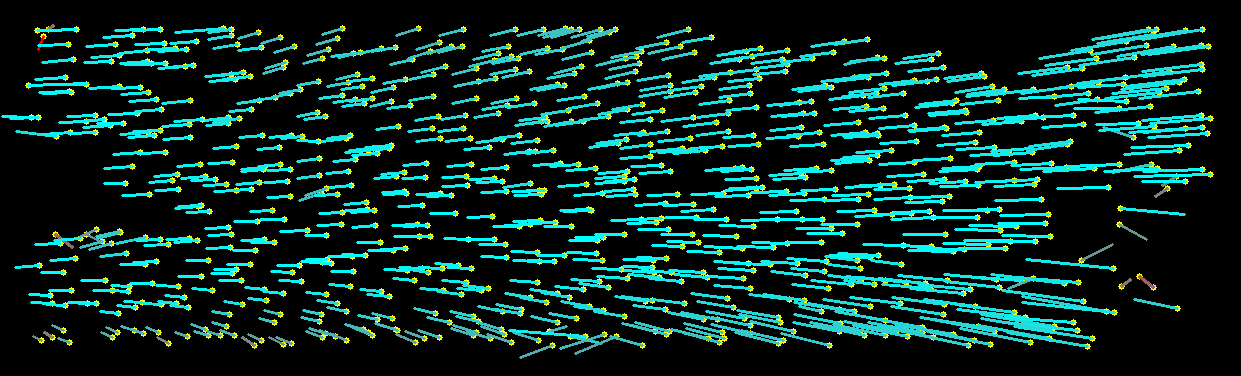
\includegraphics[width=\textwidth]{datavo/flow_196.png}
        \caption{}
        \label{fig:optical_flow_l} 
    \end{subfigure}
    \begin{subfigure}[b]{0.45\textwidth}
        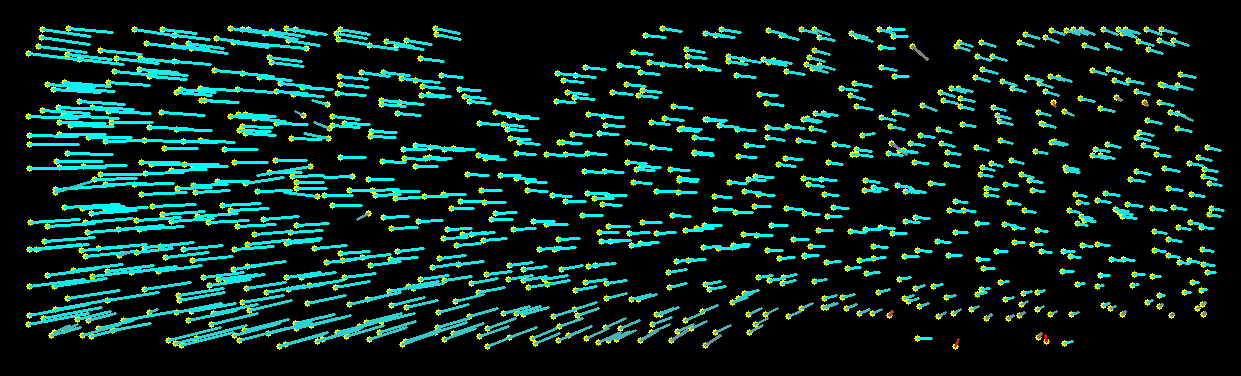
\includegraphics[width=\textwidth]{datavo/flow_96.png}
        \caption{}
        \label{fig:optical_flow_r} 
    \end{subfigure}
    \caption{路面车辆光流. (a) 向前移动时的光流; (b) 左转时的光流; (c) 右转时的光流.}
    \label{fig:optical_flow}
\end{figure}

模型的输入是堆叠的灰色图像对,我们不仅使用连续图像来构造图像对{(帧间隔为0)},而且会从{[-4,4]}中为每个样本随机选择一个{帧间隔},以此作为一个数据{增强}的过程。
输出的是相应的由y轴旋转$\theta$和{重映射}前向位移$z'$所代表的主体相机运动。$z'$是基于\eqref{eq:decouple_z}得到的。L2损失被用作监督。

\begin{equation}
    L_2 = \|\theta_g -\theta_p\|_2 +\|z'_g -z'_p \|_2
\end{equation}
下标$\theta_p$和{$z'_p$}代表预测的结果,$\theta_g$和$z'_g$代表ground truth值。
我们使用ADAM\cite{kingma2014adam}来优化模型参数,学习率设置为0.001,50个epoch后线性衰减。%我们将权重衰减参数设置为0.001以加入正则化。

模型训练完成后,以新的图像序列为输入,从模型的输出中可以得到旋转角度$\theta$和前向运动{$z'$}。
我们首先使用公式\eqref{eq:r_t_ratio}{计算平移角} $\alpha$,并假设关于其他轴的旋转为零,构建旋转角矩阵$\mathbf{R}_\theta$和$\mathbf{R}_\alpha$,则车辆转换向量
{$\mathbf{t}_\alpha=\mathbf{R}_\alpha(0,0,z')^T$}。{(这个方程等价于公式\eqref{eq:car_angle},这个过程被称为运动恢复)}。完整的车辆运动矩阵为: 
\begin{equation}
    \mathbf{T}_i =\begin{pmatrix} \mathbf{R}_\theta & \mathbf{t}_\alpha\\ 0 & 1  \end{pmatrix} 
    \label{eq:rt_final}
\end{equation}
车辆位姿通过以下公式进行累积计算:
\begin{equation}
    \mathbf{P}_i = \mathbf{P}_{i-1}\mathbf{T}_i
    \label{eq:pose}
\end{equation}

\section{实验}
\label{sec:experiments}


我们进行了四个实验来评估所提出的方法在KITTI数据集\cite{geiger2012kitti}上的性能。首先,我们描述了评估数据集和实验平台。其次,我们详细介绍了四个实验:姿势转换评估、运动
解耦性能、自我运动估计改进以及与其他方法的比较。最后,我们对实验结果进行讨论和分析。

\subsection{数据集和平台}。

KITTI\cite{geiger2012kitti}数据集提供了22个测试序列,其中前11个序列是与位姿ground truth进行评估。 在每个测试序列中提供了{RGB图像、灰色图像和激光雷达点云}。
训练和测试我们的模型时,我们只利用单目灰色图像与地面位姿ground truth{(KITTI数据集序列00-10)}。

我们划分了四个不同的训练-评估分组用于定量评估所提出的运动聚焦和解耦对自我运动估计的改进,详细内容见节\ref{sec:ego_improvement};为了与其他相对方法进行比较,在章节
\ref{sec:compare}中,我们使用KITTI-00至KITTI-08进行训练,KITTI-09和KITTI-10进行评估,这与其他基于学习的方法是一样的,以便进行公平比较。 
我们使用RPE(relative pose error,相对姿势误差)的平均值包括相对旋转误差和相对位移误差\cite{geiger2012kitti}作为评价指标。

{我们的算法是基于Python语言的PyTorch实现的,PyTorch是一个可靠的深度学习框架,具有方便的Python接口}。
我们的代码已经公开在网上,该算法在一个笔记本电脑上测试,其内存为16GB,CPU为Intel Core i7-7700 @ 2.80GHz,主频为1.5GHz。
Nvidia 1060 GPU,6GB图形内存。测试环境为Ubuntu 18.04,使用CUDA 10.0和Python 3.6.9。模型训练只需要2.0G GPU内存{当批量大小设置为30},并且在测试期间只有CPU的情况下,预测频率高于200{帧/秒}。


\subsection{实验结果}。
首先,在第\ref{sec:info_loss}节中,通过测试其RPE我们评估由运动聚焦引起的姿势位移。第二,在第\ref{sec:info_decouple}节中,我们评估了运动解耦后姿势位移的改善。
第三,在第\ref{sec:ego_improvement}节中,我们评估了所提出的运动聚焦和解耦对自我运动估计的改进。
最后,我们在第\ref{sec:compare}节中将我们的结果与其他基于学习和基于几何的方法进行比较。

\subsection{运动聚焦的运动位移}。
\label{sec:info_loss}。

%由于地面飞行器的运动受其动力学和机械结构的限制,其大部分运动是沿z轴和绕y轴的。
为了说明运动聚焦的可行性,我们定量地评估了运动聚焦的程度。
当忽略部分或所有其他无关紧要的运动维度时,姿态将发生漂移。 
我们重建了运动减少后的姿势,并利用RPE\cite{geiger2012kitti}来评估姿势位移。 {KITTI序列00-10的平均RPE记录在表\ref{tab:info_loss_1}}中。 
\begin{table}[h]
    \caption{Average RPE When Only Keeping Part of Vehicle Motion}
    \label{tab:info_loss_1}
    \begin{center}
    \begin{tabular}{c c c c c}
    \toprule
    % \hline
    \multirow{2}*{R / t} &{z}&{c}{xz}&{yz}&{zyz}\\
    & RPE(\%) /NID& RPE(\%) /NID& RPE(\%) /NID& RPE(\%) /NID\\
    %  % \hline%\hline
    \midrule
     y   &2.20  /4 & 2.06 /3 & 2.45 /3 & 2.34 /2 \\
     xy  &1.92  /3 & 1.77 /2 & 1.76 /2 & 1.56 /1 \\
     zy  &2.05  /3 & 1.91 /2 & 1.47 /2 & 1.27 /1 \\
     xyz &1.92  /2 & 1.81 /1 & 0.49 /1 & 0    /0   \\
    % \hline
    \bottomrule
    \end{tabular}
    \end{center}
 \end{table}
 \iffalse
 \begin{table}[t]
    \caption{Information Loss by Focusing only on translation along $z$ and roation about $y$}
    \label{tab:info_loss_2}
    \begin{center}
    \begin{tabular}{c c c c c c c c c c c c }
    \toprule
    % \hline
    seq & 00 & 01 & 02 & 03 & 04 & 05 & 06 & 07 & 08 & 09 & 10\\
    %  % \hline%\hline
    \midrule
     RPE(\%) &1.31 & 1.93 & 3.05 & 2.80& 2.22&1.30&1.34&1.19&1.44&3.79&3.85 \\
     ATE(m) &1.31 & 1.93 & 3.05 & 2.80& 2.22&1.30&1.34&1.19&1.44&3.79&3.85 \\
    % \hline
    \bottomrule
    \end{tabular}
    \end{center}
 \end{table}
\fi
\begin{figure}[ht]
    \centering
    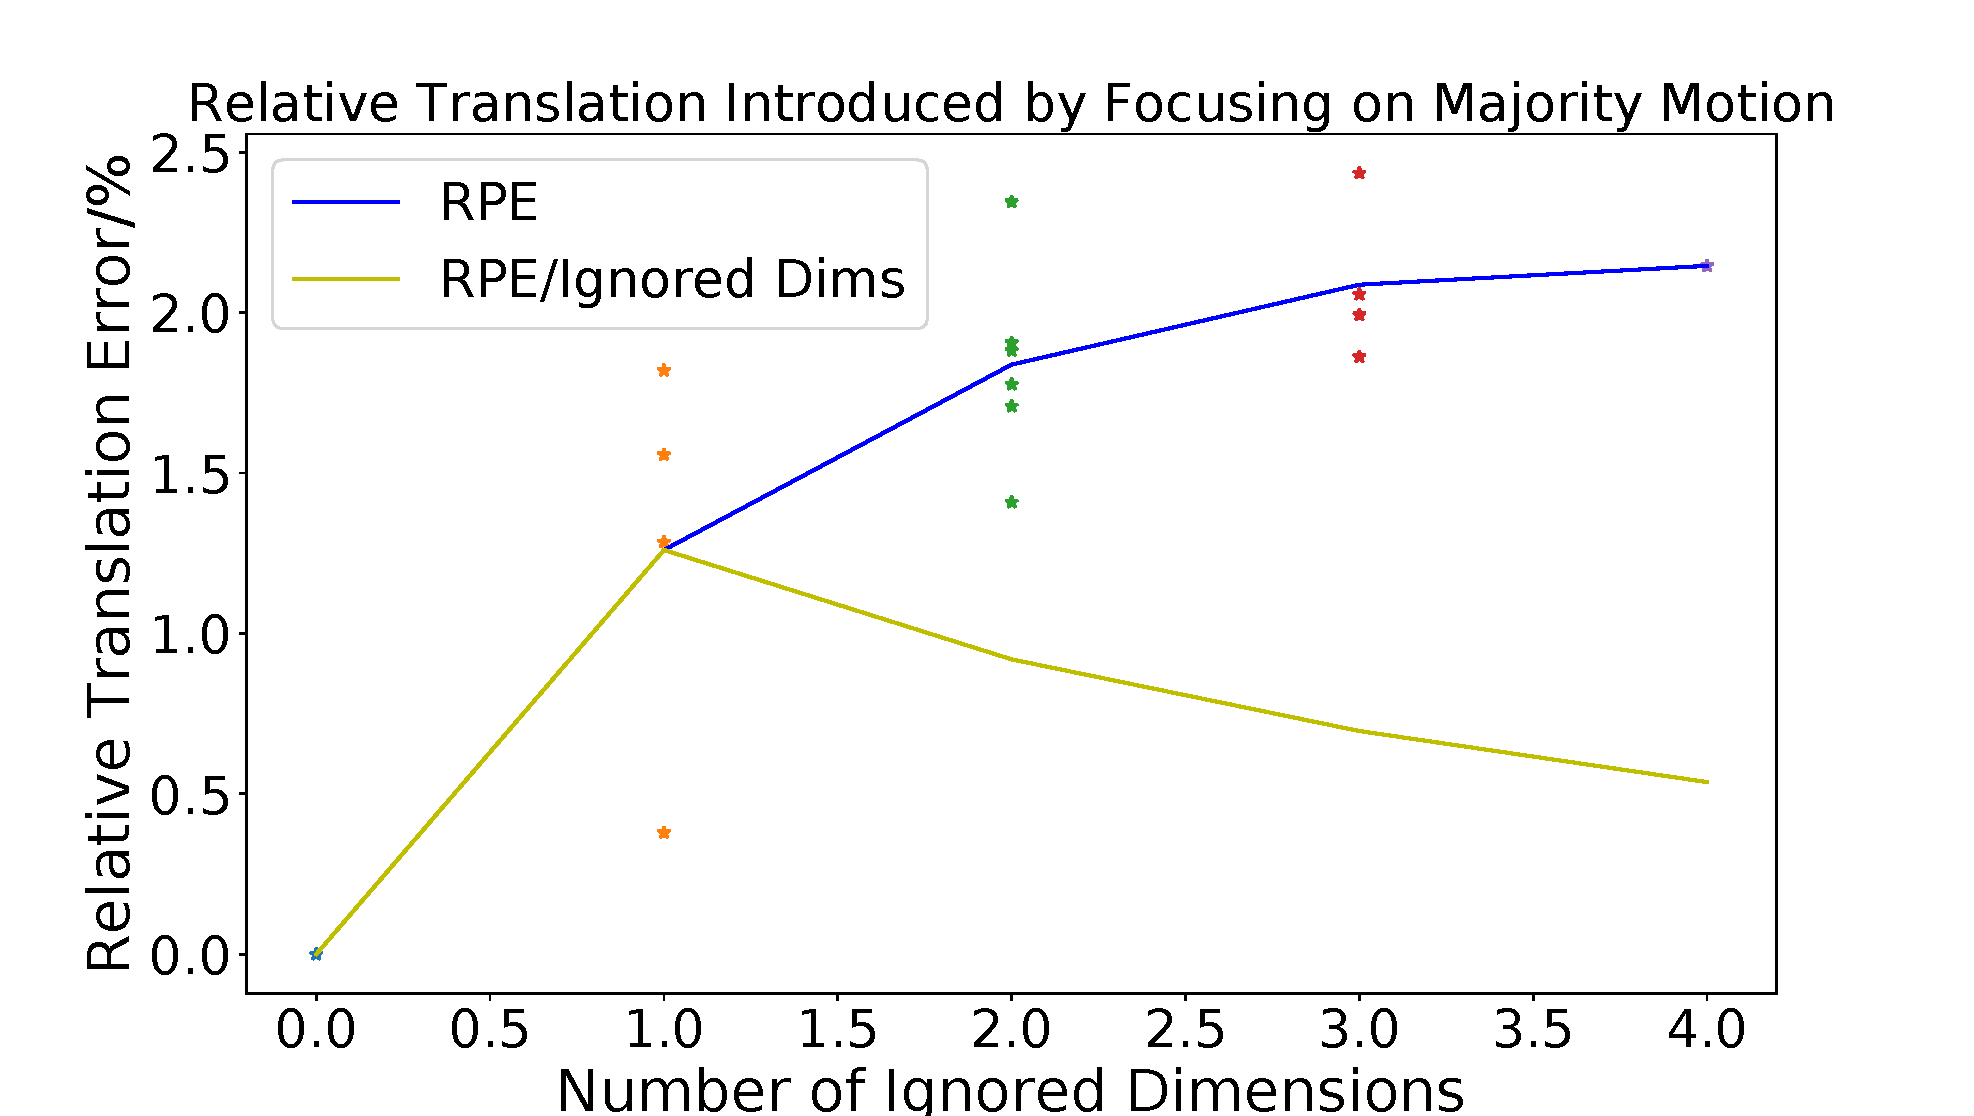
\includegraphics[width=0.46\textwidth]{datavo/info_loss.pdf}
    \caption{忽略不同的维度时RPE平均值对比。}
    \label{fig:info_loss}
\end{figure}

在表\ref{tab:info_loss_1}中,列头和行头名称分别代表保留的旋转轴和转换轴。NID是忽略的维度数( the number of ignored dimensions)的英文缩写。
当我们只保留z轴平移和y轴旋转时,重建路径的RPE为2.20\%,NID为4,我们将运动聚焦后的一些重建路径可视化,如图\ref{fig:path_recon}所示,可以看出重建后的水平路径位移误差
很小,在可接受范围内。位移主要积累在z轴上。z轴上的位移取决于运行环境,如有起伏时,位移会比较大(如图中\ref{fig:conc_10}中的序列10),环境几乎平坦时,位移较小(图中
\ref{fig:conc_07}中的序列07)。

\begin{figure}[ht]
    \centering
    \begin{subfigure}[b]{0.47\textwidth}
    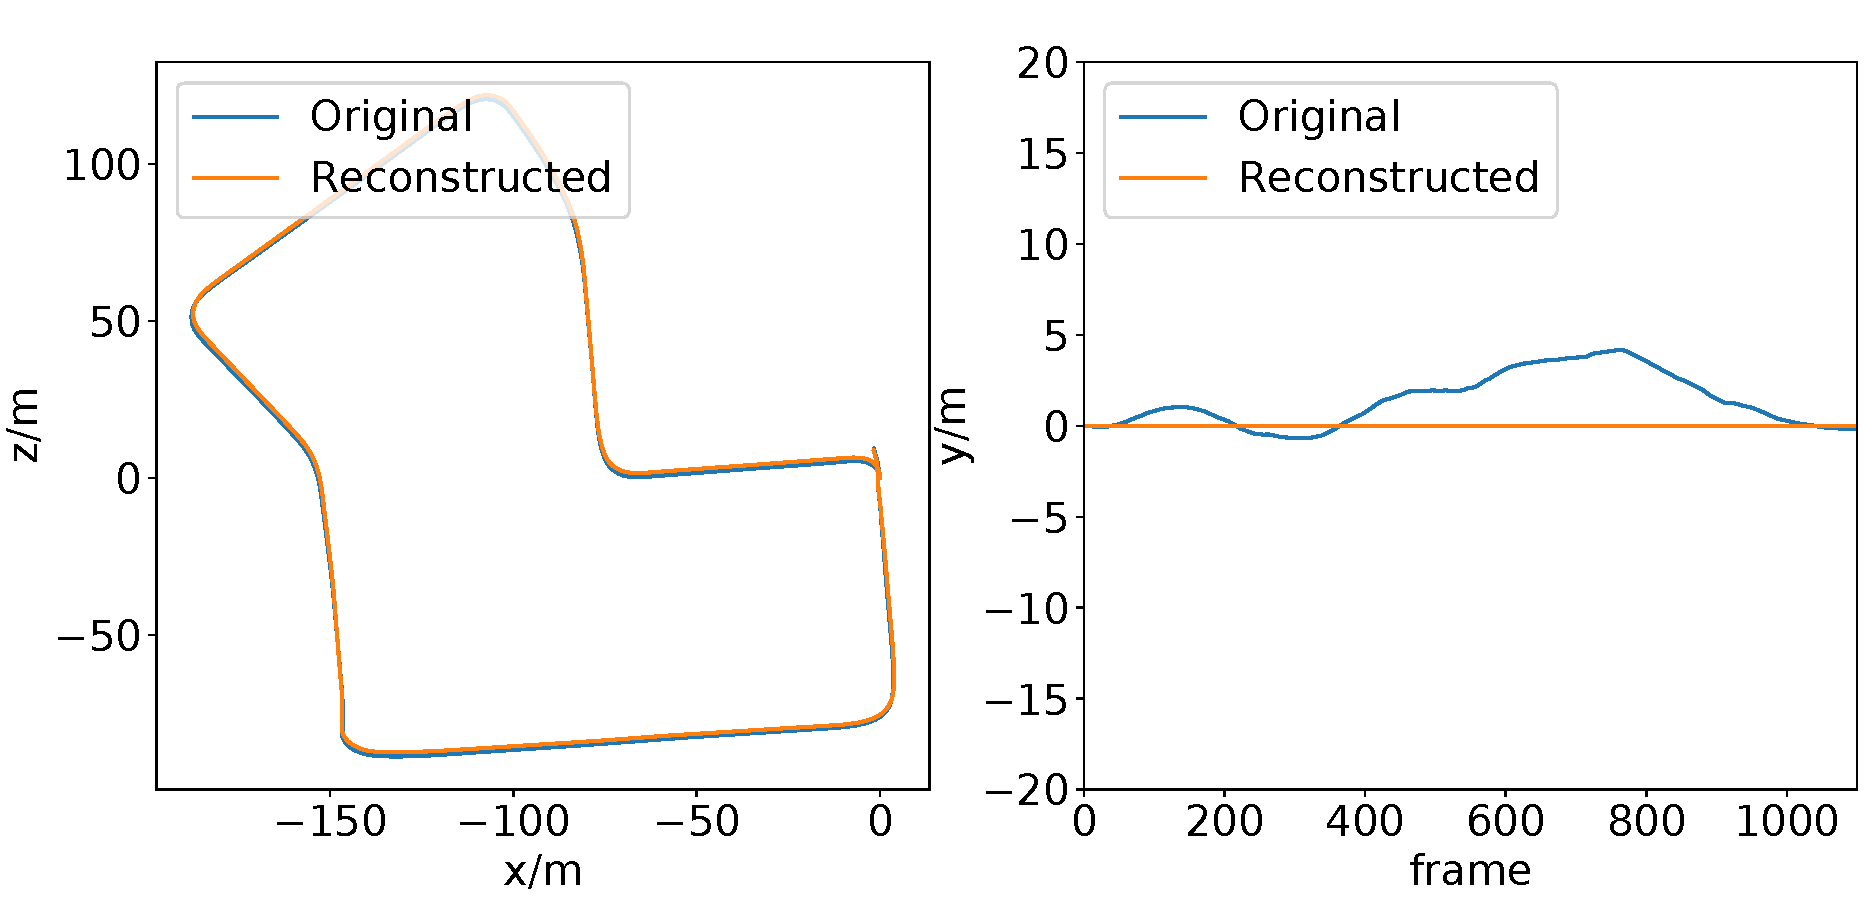
\includegraphics[width=\textwidth]{datavo/path_recon_07.pdf}
    \caption{}
    \label{fig:recon_07}
    \end{subfigure}
    \begin{subfigure}[b]{0.47\textwidth}
        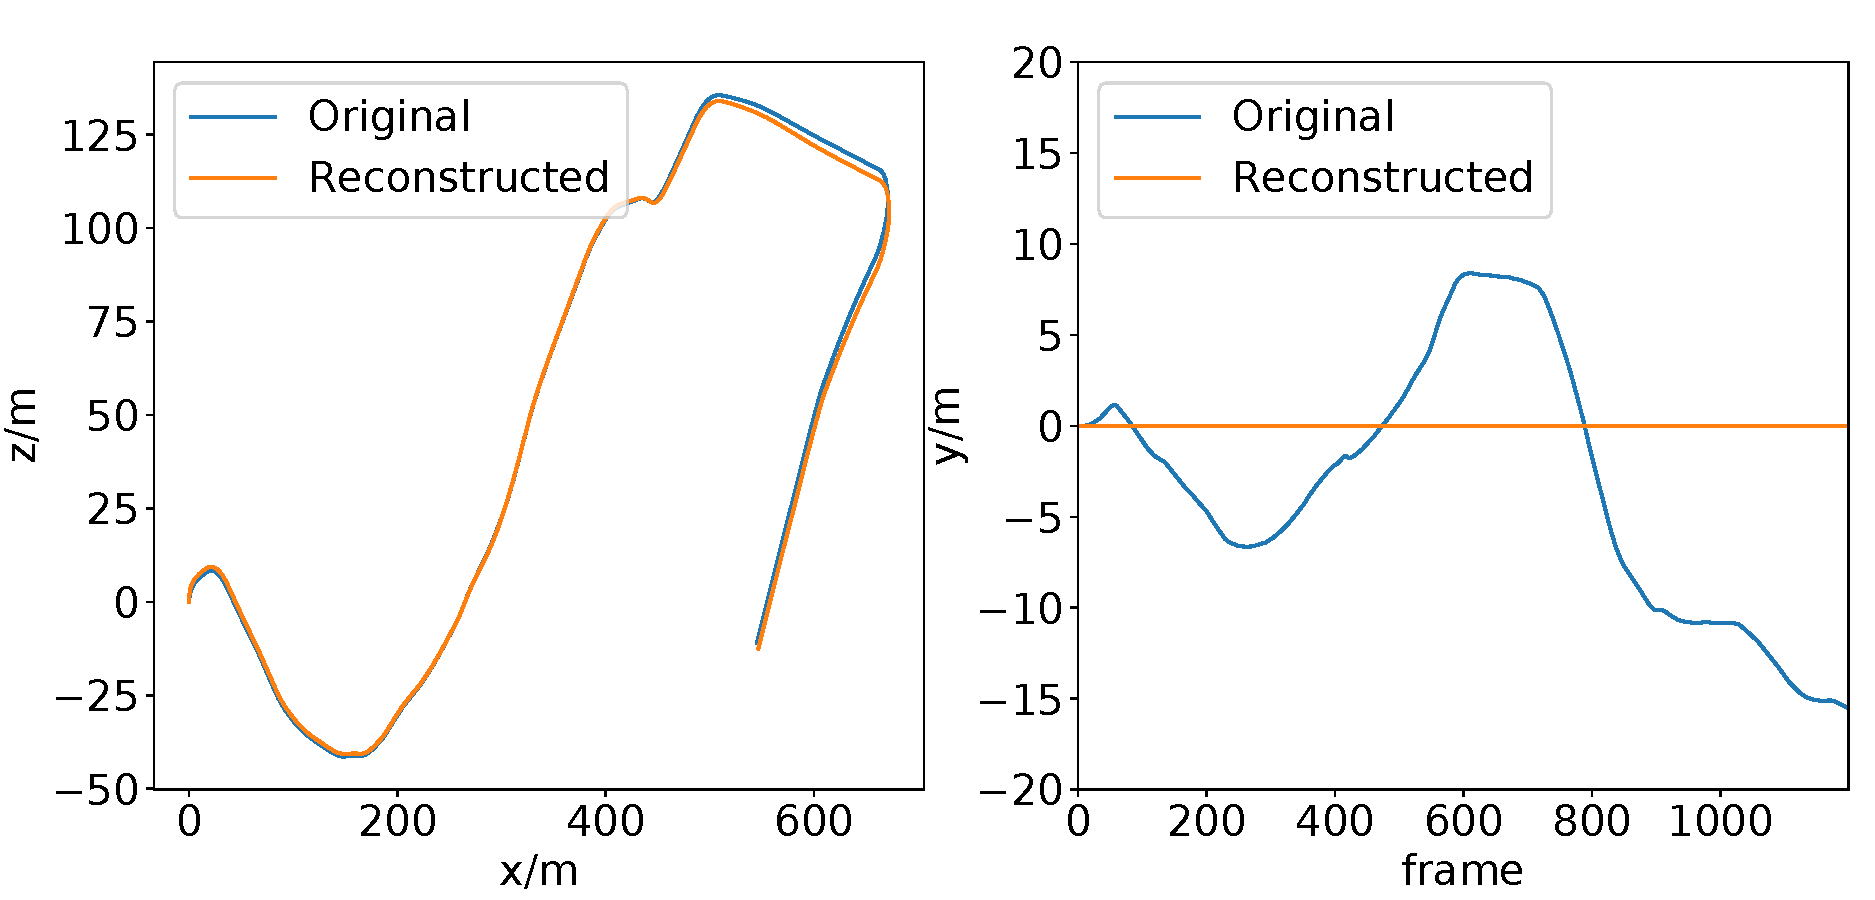
\includegraphics[width=\textwidth]{datavo/path_recon_10.pdf}
        \caption{}
        \label{fig:recon_10}
    \end{subfigure}
    \caption{恢复出的机器人路径的可视化。 (a) KITTI-07的恢复路径; (b) KITTI-10的恢复路径。} 
    \label{fig:path_recon}
\end{figure}
为了更好的理解,我们还在图\ref{fig:info_loss}中可视化了RPEs。蓝色线代表不同的忽略维度数被忽略时的平均{RPEs}。我们用忽略维度的数量(收益)去除平均RPE(成本)获得的比率
作为损失指标,由图\ref{fig:info_loss}中的黄线所示。当只保留z轴平移和y轴旋转时,成本-收益比率比相对较小。

\subsection{通过运动解耦改善姿势位移}
\label{sec:info_decouple}
为了显示所提出的运动解耦的效率,我们定量评估了运动解耦所减少的姿态位移。如表\ref{tab:info_loss_1}的第一行所示,忽略X轴的平移将导致更多的姿势位移。%(从2.06{\%}升到2.20{\%})。
运动解耦的目标是减少忽略x轴平移时的姿势位移,其方法将在章节\ref{sec:motion_decouple}中描述。

根据\eqref{eq:r_t_ratio},平移角$\alpha$和旋转角$\theta$之间的关系是线性的。然而,线性映射的斜率不是固定的,而是相对于不固定的前向运动$z$而言的。
为了简化问题,我们首先使用固定斜率参数来变换所有的前向运动,并测试不同比例的RPE,结果如图\ref{fig:static_decouple}所示。当比值设为1.7时,我们得到的RPE最小。当车辆处于旋转状态时,车辆的平均前移距离约为$\frac{1.7-0.5}{l}$米。
为了更好地理解条形图(图\ref{fig:static_decouple}),我们使用不同的颜色来表示特定的条形。
当平移-旋转角比为零时(图\ref{fig:static_decouple}中的红色条形图,RPE约为2.20,这就是没有运动解耦时的误差。
青色条对应的是平移角和旋转角相等,这是简单解耦的性能如公式\ref{eq:frlt}所示。
黑条对应的是平移偏角为旋转角度的一半,这种情况仅在相机安装在后轴中心时才成立,但相机距离后轴中心相比于车辆前进距离较小时,此系数也可近似成立\cite{scaramuzza2009real}。
\begin{figure}[ht]
    \centering
    \begin{subfigure}[b]{0.45\textwidth}
        \centering
        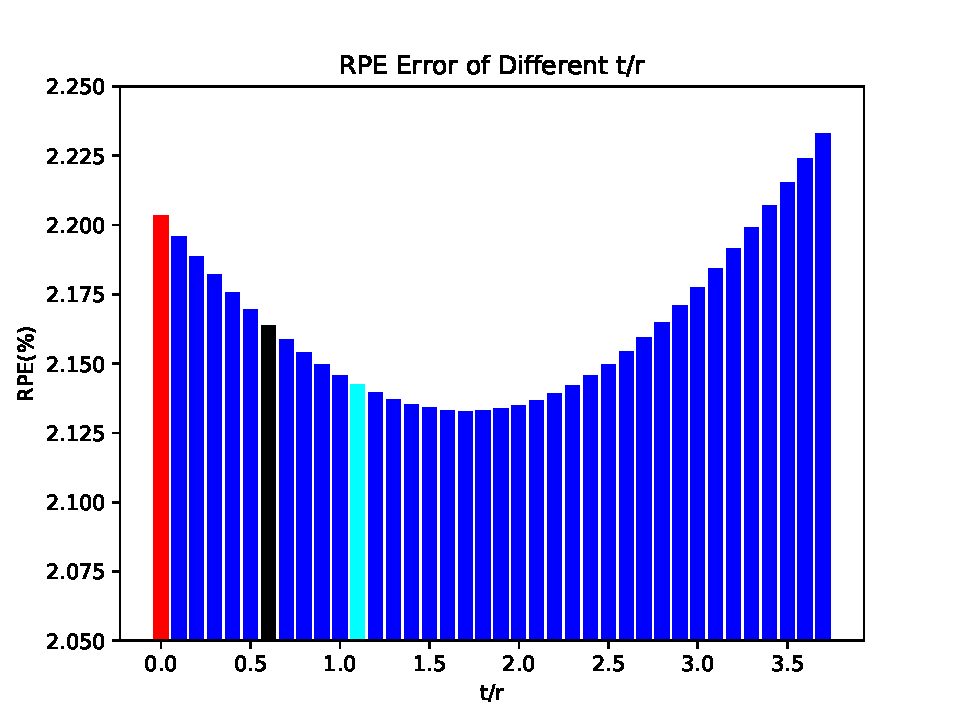
\includegraphics[width=0.9\textwidth]{datavo/r_t_ratio.pdf}
        \caption{}
        \label{fig:static_decouple}
    \end{subfigure}
    \begin{subfigure}[b]{0.45\textwidth}
        \centering
        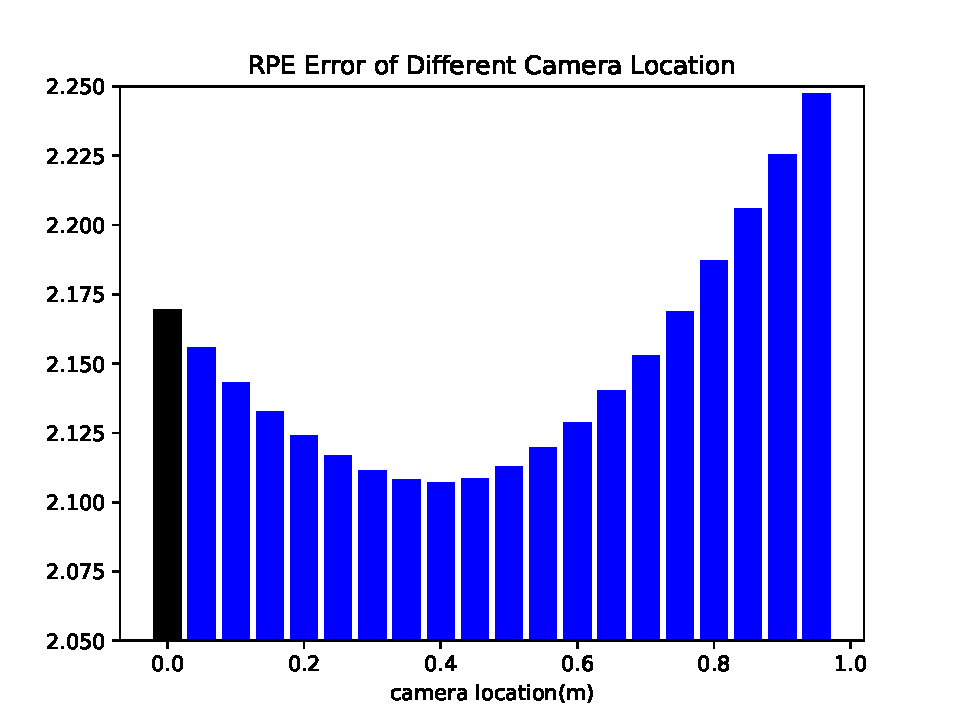
\includegraphics[width=0.9\textwidth]{datavo/r_t_ratio_2.pdf}
        \caption{}
        \label{fig:dynamic_decouple}
    \end{subfigure}
    \caption{Decoupling performance {visualization}. (a) Different fixed ratio; (b) Different dynamic ratio}.
    \label{fig:r_t_ratio}
\end{figure}


固定的比率会忽略车辆前行距离的影响,我们也尝试使用动态比率。我们测试不同的摄像头位置$l$,用公式\eqref{eq:r_t_ratio}计算比率,然后评估重建路径的RPE,如图\ref{fig:dynamic_decouple}所示。

当摄像头位置设置为距离后轴0.4m时,RPE误差最小。图\ref{fig:dynamic_decouple}中的黑条也代表着平移角$\alpha=0.5\theta$,这与图\ref{fig:static_decouple}中的黑条相同。

图\ref{fig:decouple}中可以直观地看到动态解耦和静态解耦的比较。
在图\ref{fig:decouple}中,蓝色条形代表没有运动解耦的RPE,黄色和绿色条形分别代表静态解耦(比例设为1.7)和动态解耦(摄像机位置$l$设为0.4m)的RPE,红色条形代表我们同时
保持x轴和z轴平移运动时的RPE。可以发现,无论是动态解耦还是静态解耦都可以降低RPE;当我们同时保持x轴平移和z轴平移时,动态解耦的RPE比静态解耦的RPE低。

\begin{figure}[ht]
    \centering
    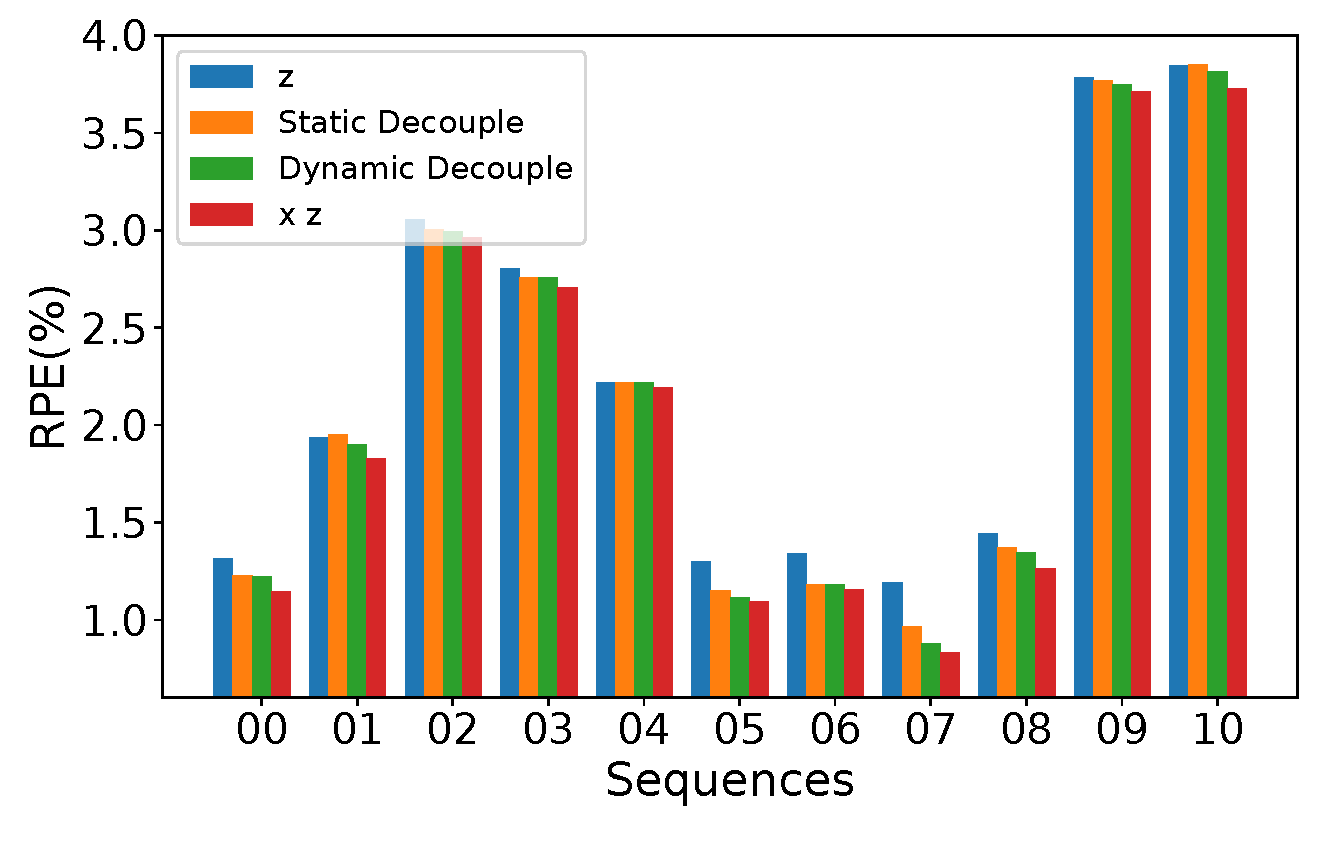
\includegraphics[width=0.45\textwidth]{datavo/decouple-crop.pdf}
    \caption{固定解耦比率与动态解耦比率的性能比较。}
    \label{fig:decouple}
\end{figure}
\subsubsection{运动聚焦与解耦后的性能提升。}

\label{sec:ego_improvement}
\begin{table}[ht]
    \caption{The improvement of motion focusing}
    \label{tab:info_improve}
    \begin{center}
    \begin{tabular}{c c c c c c }
    \toprule
    % \hline
    \multirow{3}*{Train} & \multirow{3}*{Test} &\multicolumn{2}{c}{Learn All Motion} & \multicolumn{2}{c}{Learn $R_y, t_z$}\\
    & &Trans & Rot & Trans & Rot\\
    & & (\%) & (deg/m)  & (\%) & (deg/m)\\
    %  % \hline%\hline
    \midrule
     00 & 02 04 06 08 10 &26.8 & 0.137 & 23.9 & 0.110 \\
     00 02 & 04 06 08 10 &18.3 & 0.095 & 16.7 & 0.070 \\
     00 02 04 & 06 08 10 &17.6 & 0.091 & 16.9 & 0.076 \\
     00 02 04 06 & 08 10 &15.3 & 0.082 & 13.2 & 0.065   \\
    % \hline
    \bottomrule
    \end{tabular}
    \end{center}
 \end{table}


实验研究运动聚焦和解耦的影响,我们使用相同的训练数据来训练两种模型。
1)MFM(运动聚焦模型):只学习y轴旋转和z轴平移;2)AMM(全运动模型):学习所有的六自由度运动。同一测试集上的RPE可以作为性能改进的指标。

为避免实验偶然性,实验是在不同的训练与测试数据分组上进行的。我们记录了训练集的损耗变化曲线和测试集的{RPE}。
如图\ref{fig:training_loss}所示。对于所有的训练分割,MFM模型比{AMM}模型收敛更快。
\begin{figure}[ht]
    \centering
    \begin{subfigure}[b]{0.225\textwidth}
        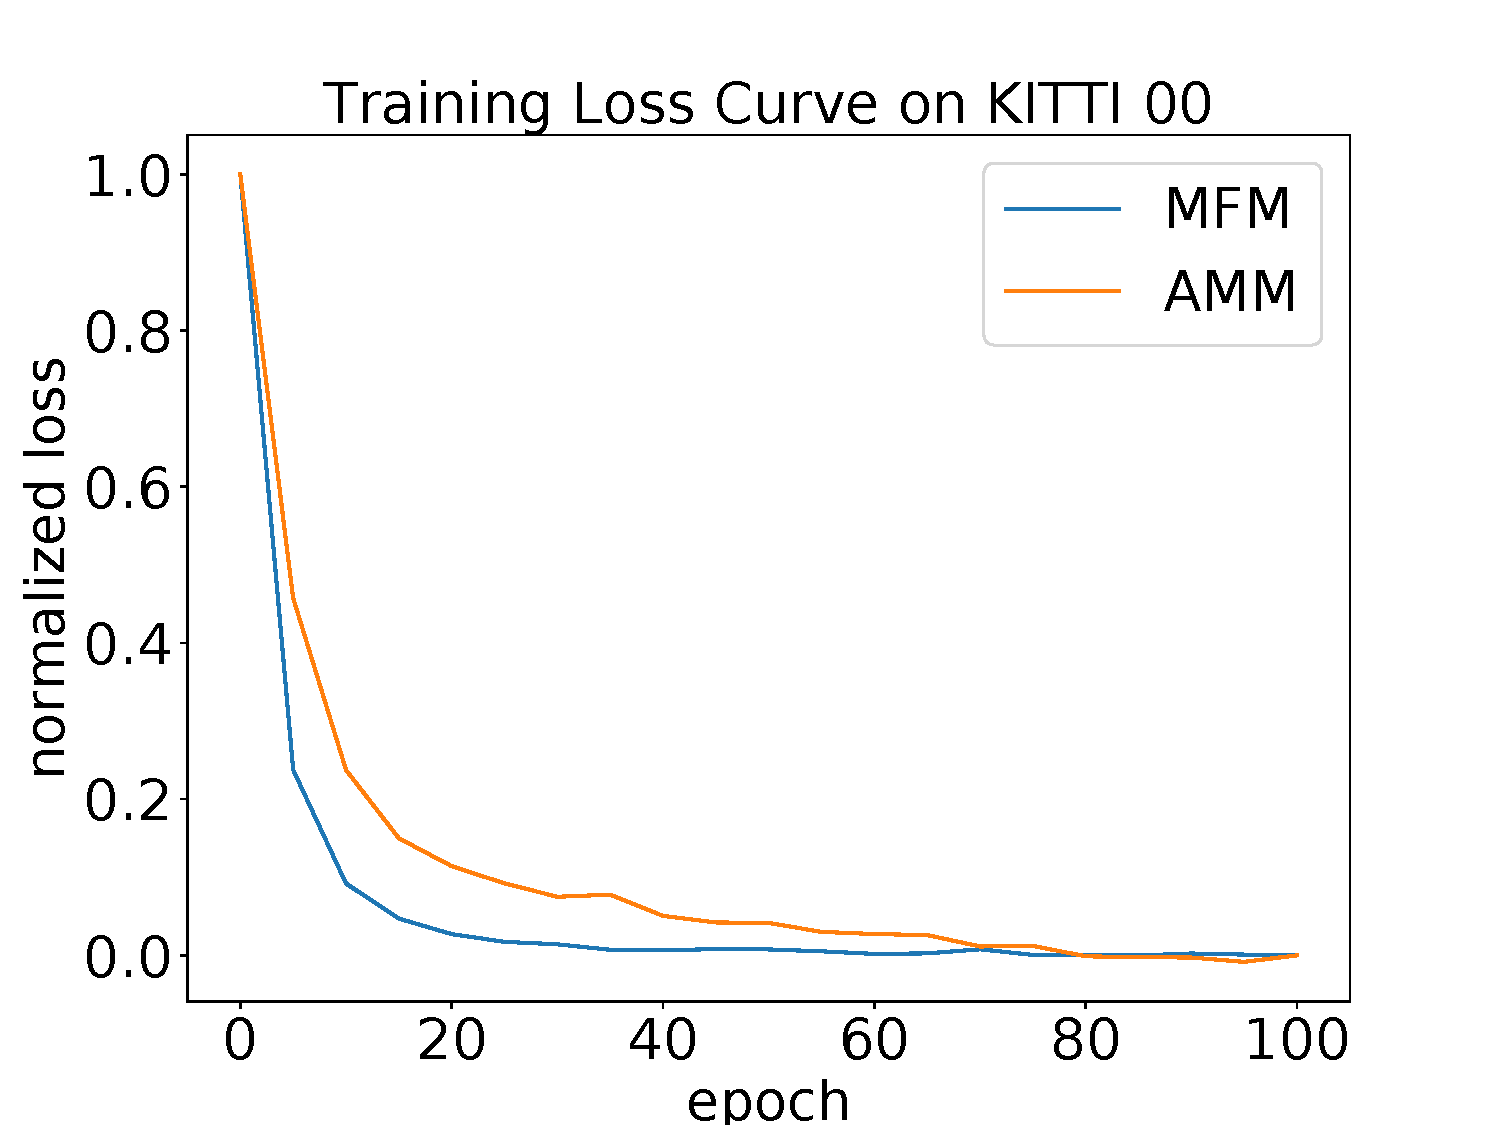
\includegraphics[width=\textwidth]{datavo/training_loss_0.pdf}
        \caption{}
        \label{fig:tl_0}
    \end{subfigure}
    \begin{subfigure}[b]{0.225\textwidth}
        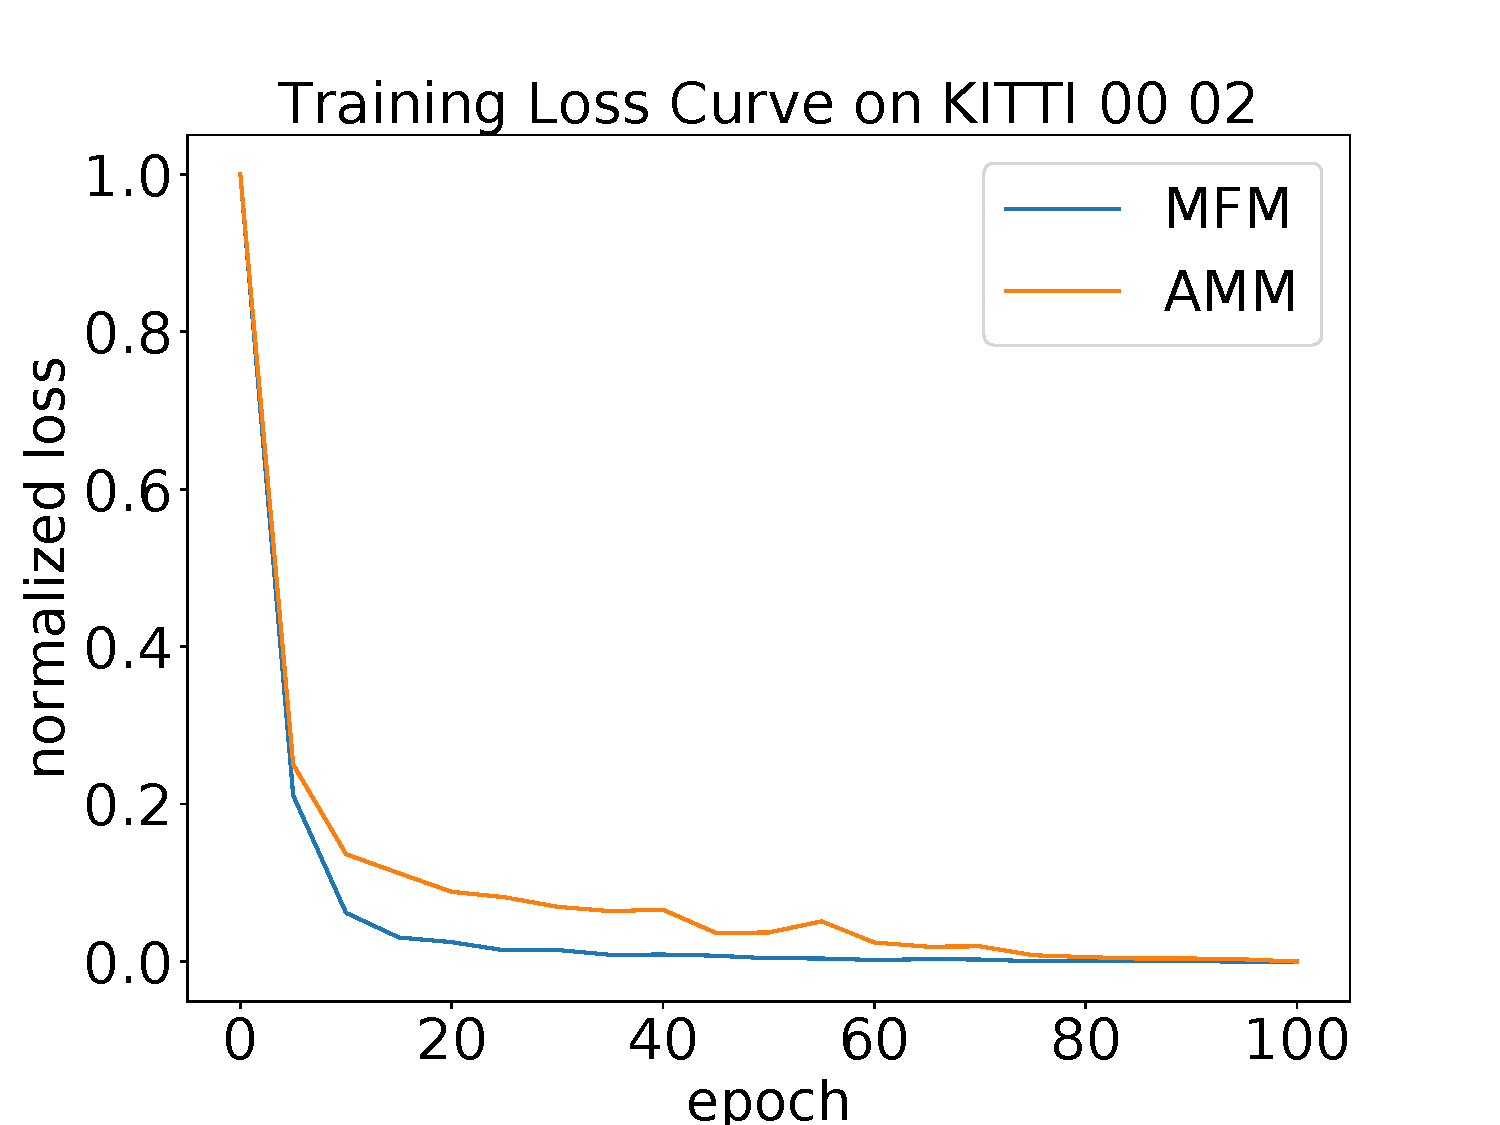
\includegraphics[width=\textwidth]{datavo/training_loss_0-2.pdf}
        \caption{}
        \label{fig:tl_02}
    \end{subfigure}
    \begin{subfigure}[b]{0.225\textwidth}
        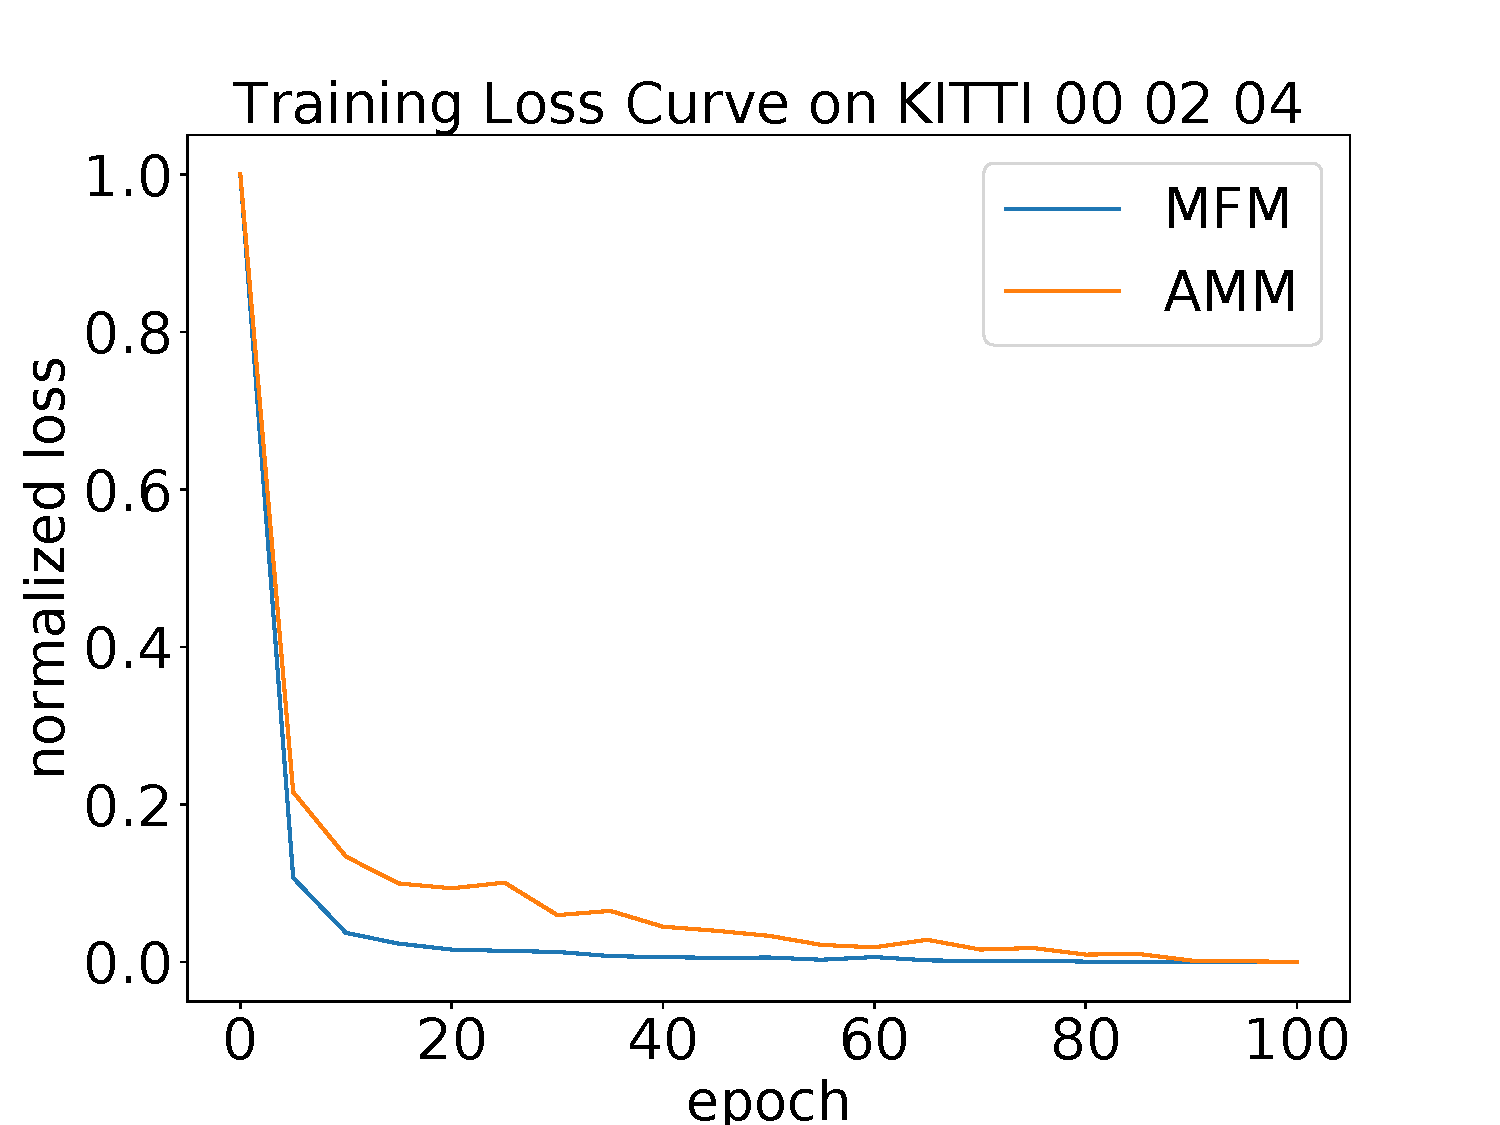
\includegraphics[width=\textwidth]{datavo/training_loss_0-4.pdf}
        \caption{}
        \label{fig:tl_024}
    \end{subfigure}
    \begin{subfigure}[b]{0.225\textwidth}
        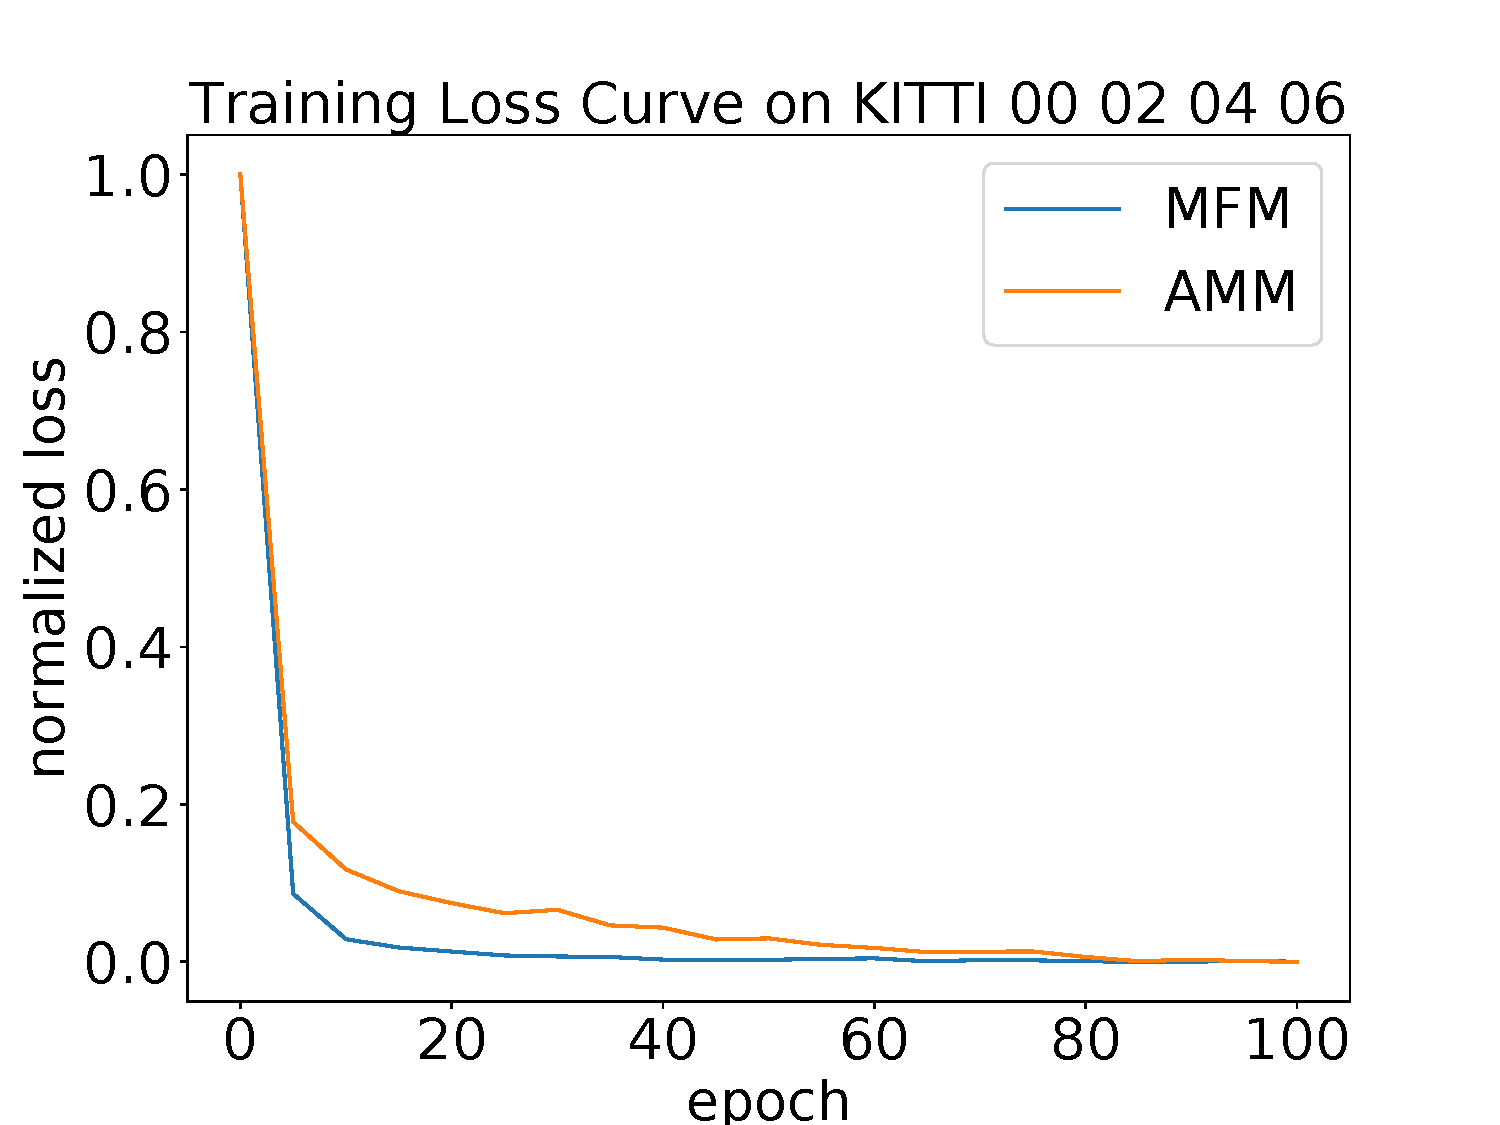
\includegraphics[width=\textwidth]{datavo/training_loss_0-6.pdf}
        \caption{}
        \label{fig:tl_0246}
    \end{subfigure}
    \caption{训练损失函数比较。(a) KITTI-00; (b)KITTI-00和KITTI-02; (c) KITTI-00,KITTI-02和KITTI-04; (d) KITTI-00,KITTI-02,KITTI-04和KITTI-06。}
    {\label{fig:training_loss}}
\end{figure}

\begin{figure}[ht]
    \centering
    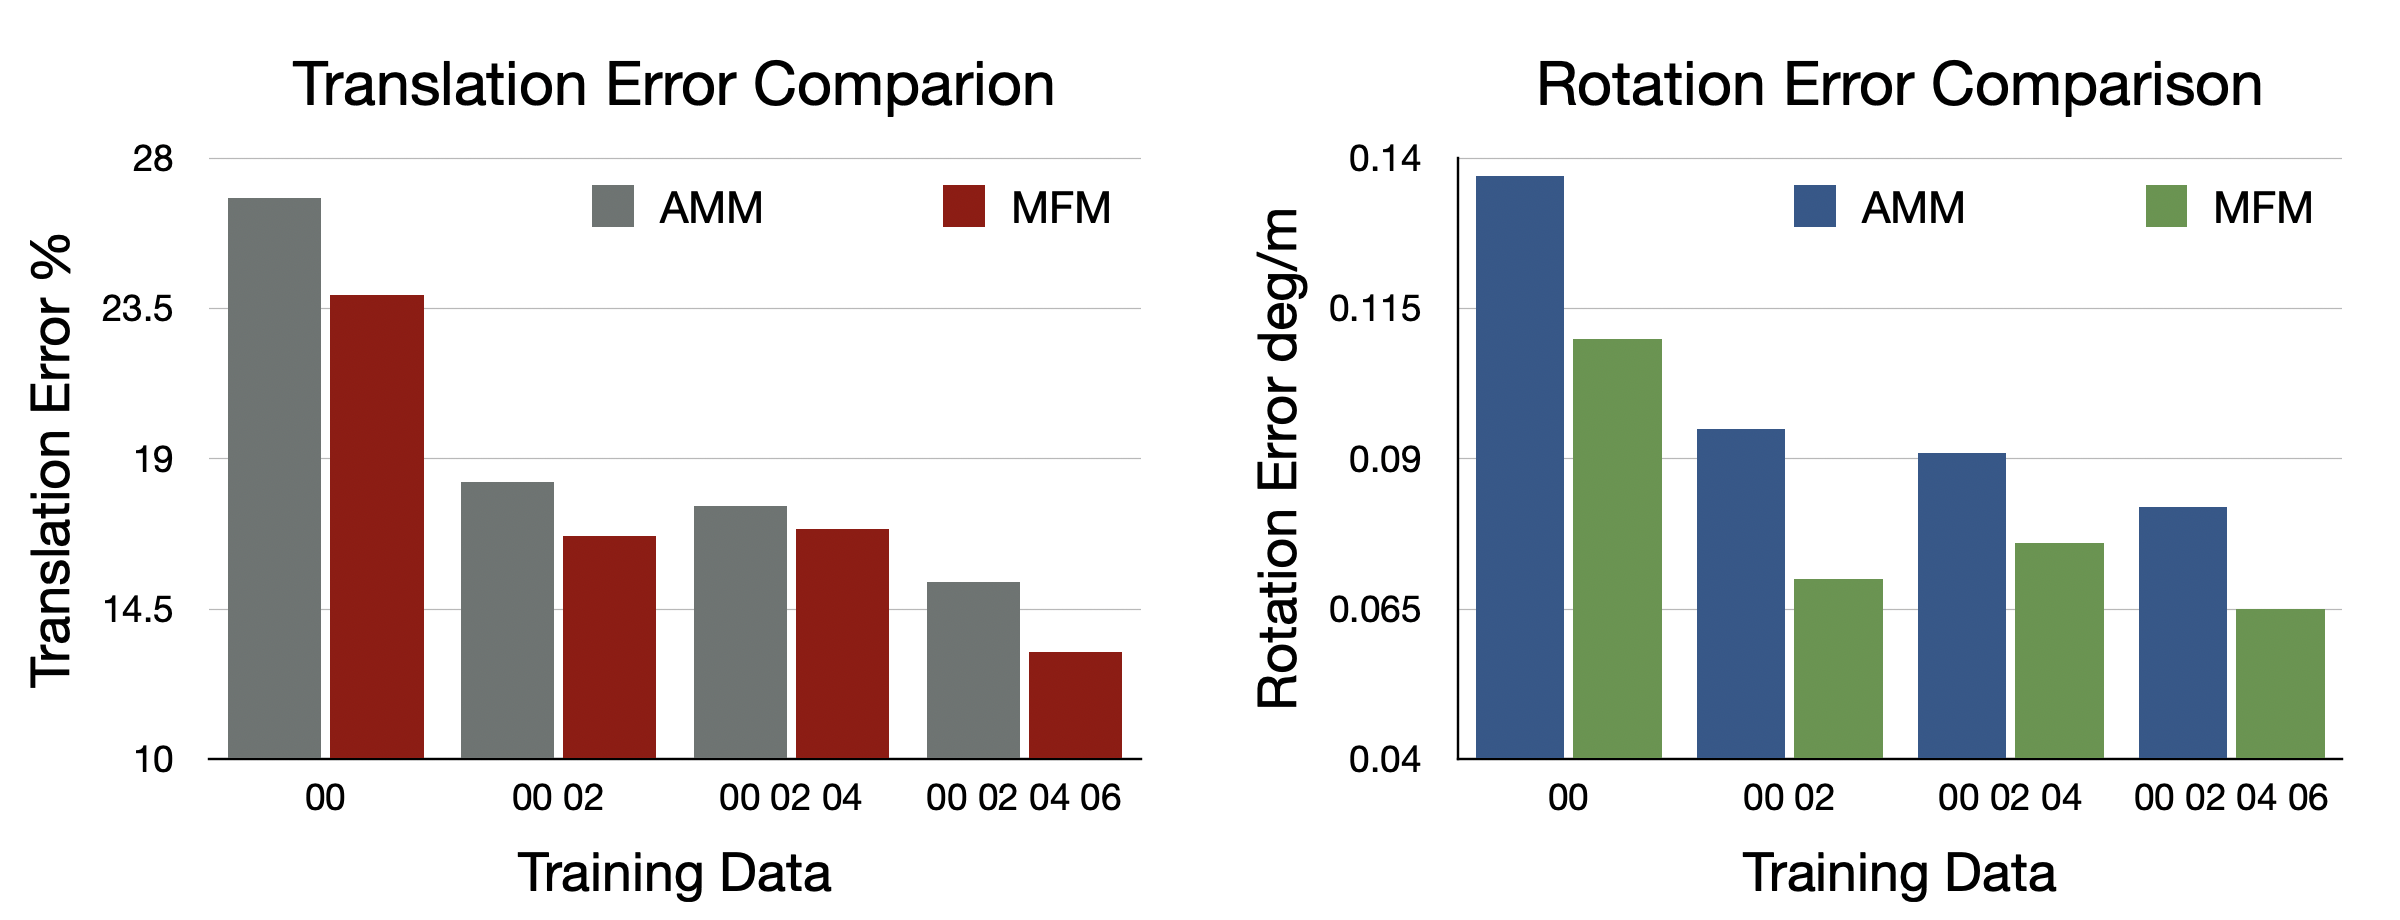
\includegraphics[width=0.45\textwidth]{datavo/focusing_train.png}
    \caption{运动聚焦训练后性能的提升。}
    \label{fig:focucing_train}
\end{figure}


不同训练模型的测试RPE记录在表\ref{tab:info_improve}中,并直观地显示在图\ref{fig:focucing_train}中。我们可以发现,运动聚焦模型的结果比所有训练分割的运动模型的结果都要好,翻译误差提高了约2\%,旋转提高了0.2度/m。值得注意的是,运动聚焦模型是由带有漂移姿势的地面真实数据{运动聚焦和解耦后}进行训练的,但测试性能仍然较好。
从测试结果中还可以观察到,随着训练数据的增加,运动聚焦模型和所有运动模型的测试效果都越来越好。
\subsection{与其他方法的比较}
\label{sec:compare}
\begin{table*}[!htbp]
    \caption{Comparison with other Learning-based Methods}
    \begin{center}
    \begin{tabular}{c c c c c c c c c c c c c c}
    \toprule
    % \hline
    \multirow{4}*{Seq} & \multicolumn{2}{c}{Zhan et al.} &\multicolumn{2}{c}{DeepVO} & \multicolumn{2}{c}{SfM-Learner.}& \multicolumn{2}{c}{GeoNet}&  \multicolumn{2}{c}{\multirow{2}*{Our Method }}\\
                       & \multicolumn{2}{c}{(from \cite{zhan2018unsupervised})}  & \multicolumn{2}{c}{(from \cite{wang2017deepvo})}&\multicolumn{2}{c}{(from \cite{zhou2017unsupervised})} &\multicolumn{2}{c}{(from \cite{yin2018geonet})} &\\
    %  % \hline%\hline
    \cline{2-3}  \cline{4-5}  \cline{6-7} \cline{8-9} \cline{10-11} \cline{12-13}
        & Trans & Rot  & Trans & Rot  & Trans & Rot &Trans & Rot& Trans & Rot\\ 
    & (\%) & (deg/m)  & (\%) & (deg/m)  & (\%) & (deg/m)& (\%) & (deg/m) & (\%) & (deg/m) \\
    \midrule
        09&11.92&0.0360&-&-&17.84&0.0678&26.93&0.0954&9.26&0.0229 \\
        10&12.62&0.0343&8.11&0.0883&37.91&0.1778&24.69&0.0843&9.10&0.0221 \\
    \midrule
    % \textbf{Avg.} & \textbf{84.0}\\
    Avg & 12.27 & 0.0351 &8.11 &0.0883  & 28.88 &0.1228 &25.81& 0.0899& 9.18&\textbf{0.0225}\\
    % \hline
    \bottomrule
    \end{tabular}
    \end{center}
    \label{tab:kitti_compare}
    \end{table*}
    
    \begin{table}[!htbp]
        \caption{Comparison with Popular Geometry-based Methods}
        \begin{center}
        \begin{tabular}{c c c c c c c c c c c c c c c c c c}
        \toprule
        % \hline
        \multirow{4}*{Seq} & \multicolumn{2}{c}{LIBVISO2} &  \multicolumn{2}{c}{ORBSLAM}& \multicolumn{2}{c}{\multirow{2}*{Our Method }}\\
                           &  \multicolumn{2}{c}{(from \cite{Song2015MoncularScale})}&\multicolumn{2}{c}{(from \cite{raul2015orb})}  &\\
        %  % \hline%\hline
        \cline{2-3}  \cline{4-5}  \cline{6-7} 
            & Trans & Rot  & Trans & Rot  & Trans & Rot\\ 
        & (\%) & (deg/m)  & (\%) & (deg/m)  & (\%) & (deg/m)& \\
        \midrule
            09&4.04& 0.0143&15.30&0.0026& 9.26&0.0229\\
            10&25.20 &0.0388&3.68&0.0048 &9.10&0.0221\\
        \midrule
        % \textbf{Avg.} & \textbf{84.0}\\
        Avg &14.62 & 0.0266& 9.49&0.0037 &\textbf{9.18}&0.0225\\
        % \hline
        \bottomrule
        \end{tabular}
        \end{center}
        \label{tab:kitti_compare_ge}
        \end{table}
    
我们将我们的性能与其他基于学习和{基于几何的}方法进行比较。我们的模型在KITTI-00至KITTI-08上进行训练,在KITTI-09和KITTI-10上进行测试,数据分割与其他基于CNN的{(CNN是卷积神经网络的简称)}方法相同\cite{zhan2018unsupervised,zhou2017unsupervised,yin2018geonet}。
测试的RPE记录在表\ref{tab:kitti_compare}和表\ref{tab:kitti_compare_ge}中。
由于SfM-Learner\cite{zhou2017unsupervised}和GeoNet\cite{yin2018geonet}的模型都是以自监督的方式进行无绝对尺度的训练,因此在评价前,它们的路径与路径ground truth经过了校准对齐。
Zhan等人的模型\cite{zhan2018unsupervised}、DeepVO\cite{wang2017deepvo}和我们的方法都是用绝对尺度训练的,所以不需要对齐。
ORB-SLAM的单目规模\cite{raul2015orb}和LIBVISO\cite{Geiger2011IV}的尺度也是与地面真实路径对齐过的。

如表\ref{tab:kitti_compare}所示,我们的方法优于基于CNN的方法(自我运动模型主要由卷积层构建)\cite{zhan2018unsupervised,zhou2017unsupervised,yin2018geonet},并与
基于CNN-RNN{(RNN是Recurrent Neural Network的缩写)}的方法\cite{wang2017deepvo}效果不相上下,后者可以临时信息优化姿势。与两种流行的传统方法LIBVISO单目法
(LIBVISO monocular \cite{Geiger2011IV}和ORB-SLAM单目法(ORB-SLAM monocular \cite{raul2015orb})比较,我们得到了最好的平移性能。


\section{讨论}

在本节中,我们将对结果进行总结,对性能进行分析,并说明所提出的方法的局限性。
\subsection{建议方法的效率}

从上面的实验结果来看,可以得出四个方面的结论。
1)运动聚焦不会带来太大的姿势位移。平均RPE只有百分之2左右,也就是说在车辆运行100米后会有2米左右的车辆姿态漂移。路径可视化显示,重建后的路误差在可接受范围。
2)运动解耦可以减少姿势位移。运动解耦利用y轴旋转和x轴平移的相关性来减少重构后的姿态位移。动态解耦的性能优于静态解耦。
对于动态解耦,需要对摄像机的位置有所要求。在上述实验中,摄像头位置是根据地面真实数据计算出来的。在实际操作中,如果你的数据是自己采集的,也可以直接测量。
3)运动聚焦{和解耦}可以从两个方面提高自我运动估计性能。首先,它缩短了训练时间,所有的训练实验都在20个纪元内收敛,但所有运动的模型在大约60个epoch后才收敛,所以运动聚焦模型与所有运动模型相比,可以减少大约2/3的训练时间。此外,尽管训练的地面真值姿势有一定的漂移{运动聚焦和运动解耦后},但{MFM}的测试性能优于{AMM}。
4)在与基于几何的方法比较的过程中,发现基于几何的方法并不稳健,在不同序列上获得的性能各异。我们的方法更加稳定和稳健,平均性能更好。我们的方法也优于其他基于CNN的方法,并可与利用RNN提高性能的DeepVO\cite{wang2017deepvo}相媲美。我们获得了更好的相对旋转性能,但平移性能比DeepVO差。


\subsection{为什么运动聚焦和解耦有效}

运动聚焦{和解耦}性能较好的原因有三点:首先,地面车辆的运动是受约束的,且分布不均衡,忽略不明显的运动不可能造成大的姿态位移,这一点已在第\ref{sec:info_loss}节中得到证明。
而这也是运动聚焦的根本基础;第二,不重要的运动太有限,没有足够的信噪比,所以模型在瞄准它们建模时,很容易被噪声干扰;第三,当我们只聚焦于二维运动时,训练任务变得{简单很多}。可以
采用轻量模型,训练数据相对充足。实验证明,增加训练数据量确实可以提高测试性能,如表\ref{tab:info_improve}所示。

\subsection{限制}

当汽车在一个近似平面空间运动时,所提出的方法可以获得更好的性能。当有明显的x轴旋转时,性能将下降。
如图\ref{fig:decouple}所示,序列09和10的RPE误差相对较高,因为在{这}两个序列中,地面车辆的运动不是{平面}的,如图\ref{fig:path_recon}所示。为了解决这个限制,一个可行的
方法是采用其他传感器,如IMU(惯性测量单元)来估计X轴的旋转,这可以作为所提出的模型所估计的平面运动的补充。

此外,另一个局限性是假设摄像机是平放且向前看的。如果摄像机有一个俯仰角,车辆的前向运动将被映射成Z轴运动和Y轴运动。在这种情况下,摄像机俯仰角$\sigma$应在训练前进行校准。然后,平移运动应该被重新定义为
\begin{equation}
    t_\sigma = \begin{pmatrix} 1 & 0 & 0 \\ 0 & \cos(\sigma) & -\sin(\sigma)\\ 0 & \sin(\sigma) & \cos(\sigma) \end{pmatrix} t
    \label{eq:pitch_correction}
\end{equation}
这些局限性也可以通过利用视觉里程测量的多模型结构来解决,每个子模型只关注地面车辆的一个维度运动,六自由度可以用六个分离的模型来学习,在这种情况下,应该考虑模型权重分摊的影响。



\section{本章小结}
本文通过提出运动聚焦和运动解耦,将地面车辆的运动制定为两个自由度的运动。实验证明了运动聚焦的可行性,并通过定量的姿态位移评估,进一步降低了姿态位移。
基于地面车辆的旋转模型,我们提出了运动解耦,进一步降低了姿势位移。我们构建了一个轻量级CNNs来对两自由度运动进行建模,它可以在CPU上实时运行。实验证明,
运动聚焦和解耦可以提高自我运动估计性能,缩短收敛时间。在KITTI数据集上与其他方法的比较表明,所提出的方法的性能与其他端到端视觉里程测量方法相当,甚至更好,
并且比基于几何的方法更稳健。

